\documentclass[11pt,letterpaper]{article}
\usepackage[margin=.7in,headheight=15pt]{geometry}
\usepackage[T1]{fontenc}\usepackage{lmodern}\pdfmapfile{+lm.map}\pdfmapfile{+cm.map}
\usepackage{amsmath,amssymb,booktabs,array,enumitem,fancyhdr,tikz,hyperref}
\usetikzlibrary{arrows.meta,positioning}
\hypersetup{colorlinks=true,urlcolor=black,linkcolor=black}
\renewcommand{\familydefault}{\sfdefault}
\setlength{\parindent}{0pt}\setlength{\parskip}{6pt}
\setlist[itemize]{label=$\bullet$,itemsep=2pt,topsep=3pt,leftmargin=16pt}
\pagestyle{fancy}\fancyhf{}\fancyhead[L]{\small Bellingham Math Circle}\fancyhead[R]{\small Polygon triangulations and flips}
\fancyfoot[L]{\small Week 14 library slot / Draft and unpiloted}\fancyfoot[R]{\thepage}
\renewcommand{\headrulewidth}{0pt}
\newcommand{\pagehead}[1]{{\Large\bfseries #1}\par\vspace{3pt}}
\newcommand{\prob}[2]{\par\vspace{5pt}{\large\bfseries #1}\par #2}
\newcommand{\hint}[1]{\par\textbf{If needed.} #1\par}
\begin{document}
\pagehead{Triangulations mathematical overview}
\textbf{Setting.} A strictly convex polygon has $n\geq3$ fixed, labeled corners. A triangulation fills it using noncrossing diagonals between original corners only. No new boundary or interior vertices are allowed. Rotating the paper does not identify different labeled fillings.

\textbf{Counts and local moves.} Every triangulation has $n-2$ triangles and $n-3$ diagonals. There are $C_{n-2}$ labeled triangulations, where $C_m=\frac{1}{m+1}\binom{2m}{m}$; the small counts are $1,2,5,14$ for $n=3,4,5,6$. Each diagonal borders two triangles forming a convex quadrilateral. Replacing it by that quadrilateral's other diagonal is a flip. Thus each triangulation has exactly $n-3$ flip neighbors.

\textbf{Global structure.} The pentagon's five triangulations form a five-cycle under flips, so an odd return route is possible. All triangulations of a fixed convex polygon are connected by flips. If $d_v$ of a triangulation's diagonals already meet corner $v$, its exact distance to the fan at $v$ is $n-3-d_v$: each flip adds at most one desired diagonal, and a sequence attaining that bound exists. Counting missing target diagonals gives only a lower bound for an arbitrary nonfan target.

\textbf{Across the bands.} K--1 constructs valid fillings, compares counts and makes one-line changes. Grades 2--3 organizes complete small collections and draws a graph whose vertices are whole triangulations. Grades 4--5 investigates odd loops, shortest routes to fans and general connectivity. The Catalan formula is adult orientation, not a required child calculation or a theorem proved in full in this packet.

\textbf{Discovery and explanation.} Let drawings suggest a count or distance conjecture. A complete classification proves a small collection is exhaustive; induction explains the triangle count; a lower bound plus a matching flip route proves a shortest distance. A route found experimentally need not be shortest. The convexity and fixed-vertex assumptions matter. Detailed proofs and solutions follow the preparation page.

\newpage
\pagehead{Polygon triangulations facilitator guide}
This guide keys the final F14-K-v2, F14-23-v2, and F14-45-v2 student packets. They have 6, 8, and 7 pages, respectively. The middle packet has seven problems; page 8 is explicitly labeled Problem 7 (continued) and provides extra hexagons for the same collection. There are 20 distinct numbered problems across the three bands. ``Week 14'' is an unscheduled library label. This guide and these activities are draft and unpiloted.

\textbf{Mathematical purpose.} Children construct complete triangle fillings, distinguish fixed-label configurations, find complete small collections, and investigate how one local change connects them. The pentagon admits a five-flip return loop. Fan targets have a useful exact distance rule. These conclusions should emerge after drawing and comparing.

\textbf{Prerequisites and entry points}
\begin{itemize}
\item K--1: point to original corners, draw or direct a straight line, recognize triangles, and compare two pictures. Adult reads and may trace. No reading, angle measurement, or multiplication is required.
\item Grades 2--3: preserve labels while comparing pictures, organize a collection, and count changes. The hexagon collection is a substantial optional endpoint.
\item Grades 4--5: track several configurations and compare a construction with a lower bound. General reasoning may be spoken and picture based. No Catalan formula, algebra, or polytope vocabulary is assumed.
\end{itemize}
\textbf{Supplies and preparation for ten children.} Prepare ten pencils, erasers, short straightedges, 20 tracing sheets, and at least 30 blank Letter sheets beyond the packets. These are proposed quantities, not an inventory claim. Print single-sided at 100\%. The large working polygons are roughly 3--5 inches across. The student polygon boards are regular, with equally scaled axes; compact copies are for recording answers. Use the larger outlines or tracing paper for the main exploration. Tracing sheets preserve printed starts and separate alternative answers. Pattern-block triangles are unsuitable: legal triangles vary in size and shape. Label every traced corner before drawing inside it.

\textbf{A flexible one hour menu}
\begin{itemize}
\item Minutes 0--4: handle tracing paper and straightedges; make lines on scrap paper.
\item Minutes 4--8: demonstrate the legal drawing action together.
\item Minutes 8--28: K--1 P1--2; middle P1--2; upper P1--2. Let children draw and compare before organizing the full collection.
\item Minutes 28--31: optional standing pause: hold up two tracings and point to the single line that changed.
\item Minutes 31--53: choose fixed-line completions, one-change neighbors, a pentagon map, or a shortest-route question. Keep middle P7 in reserve if collecting fourteen cases would displace the flips children want to explore.
\item Minutes 53--60: share a complete collection, an odd return route, or a shortest-route certificate. Stopping with one convincing example is fine.
\end{itemize}
\textbf{Whole group launch.} On a convex quadrilateral, draw one diagonal between two printed corners. Ask, ``Is the whole shape triangles now?'' Trace a copy, erase only that diagonal on the tracing, and draw the other one. Let children make the same change. Name the operation later, after they have used it. Do not show the five-cycle or the fan rule in advance.

\newpage
\pagehead{Rules and a complete pentagon collection}
\textbf{Legal fillings.} Use only straight segments between the original corners of a strictly convex polygon. No new interior points, extra edge points, moving corners, or crossing interiors. Fill the entire polygon with triangles. The labels stay attached to their corners even if the sheet turns. Two fillings differ exactly when their sets of diagonals differ. Rotations of the paper do not identify labeled fillings.

\textbf{Reading this key.} AC means the diagonal joining A and C, and a list such as AC, AD specifies the entire filling. For K--1 use $1=A,2=B,3=C,4=D,5=E,6=F$. Lists never include polygon boundary edges. In the diagrams below, $F_A$ means the fan whose two diagonals meet at A.
\begin{center}\begin{tabular}{ccccc}
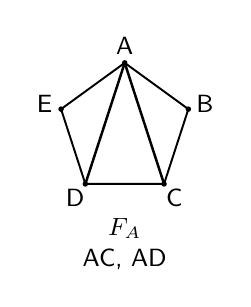
\begin{tikzpicture}[baseline=(current bounding box.center),every node/.style={font=\small}]
\coordinate (v0) at (0.0000,0.8500);
\coordinate (v1) at (0.8084,0.2627);
\coordinate (v2) at (0.4996,-0.6877);
\coordinate (v3) at (-0.4996,-0.6877);
\coordinate (v4) at (-0.8084,0.2627);
\draw[line width=.7pt] (v0)--(v1)--(v2)--(v3)--(v4)--cycle;
\draw[line width=.9pt](v0)--(v2);
\draw[line width=.9pt](v0)--(v3);
\fill (v0) circle (1pt);\node at (0.0000,1.0700) {A};
\fill (v1) circle (1pt);\node at (1.0176,0.3306) {B};
\fill (v2) circle (1pt);\node at (0.6289,-0.8656) {C};
\fill (v3) circle (1pt);\node at (-0.6289,-0.8656) {D};
\fill (v4) circle (1pt);\node at (-1.0176,0.3306) {E};
\node[align=center,font=\small] at (0,-1.450) {$F_A$\\AC, AD};
\end{tikzpicture} & 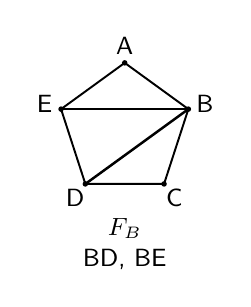
\begin{tikzpicture}[baseline=(current bounding box.center),every node/.style={font=\small}]
\coordinate (v0) at (0.0000,0.8500);
\coordinate (v1) at (0.8084,0.2627);
\coordinate (v2) at (0.4996,-0.6877);
\coordinate (v3) at (-0.4996,-0.6877);
\coordinate (v4) at (-0.8084,0.2627);
\draw[line width=.7pt] (v0)--(v1)--(v2)--(v3)--(v4)--cycle;
\draw[line width=.9pt](v1)--(v3);
\draw[line width=.9pt](v1)--(v4);
\fill (v0) circle (1pt);\node at (0.0000,1.0700) {A};
\fill (v1) circle (1pt);\node at (1.0176,0.3306) {B};
\fill (v2) circle (1pt);\node at (0.6289,-0.8656) {C};
\fill (v3) circle (1pt);\node at (-0.6289,-0.8656) {D};
\fill (v4) circle (1pt);\node at (-1.0176,0.3306) {E};
\node[align=center,font=\small] at (0,-1.450) {$F_B$\\BD, BE};
\end{tikzpicture} & 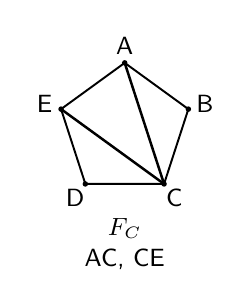
\begin{tikzpicture}[baseline=(current bounding box.center),every node/.style={font=\small}]
\coordinate (v0) at (0.0000,0.8500);
\coordinate (v1) at (0.8084,0.2627);
\coordinate (v2) at (0.4996,-0.6877);
\coordinate (v3) at (-0.4996,-0.6877);
\coordinate (v4) at (-0.8084,0.2627);
\draw[line width=.7pt] (v0)--(v1)--(v2)--(v3)--(v4)--cycle;
\draw[line width=.9pt](v0)--(v2);
\draw[line width=.9pt](v2)--(v4);
\fill (v0) circle (1pt);\node at (0.0000,1.0700) {A};
\fill (v1) circle (1pt);\node at (1.0176,0.3306) {B};
\fill (v2) circle (1pt);\node at (0.6289,-0.8656) {C};
\fill (v3) circle (1pt);\node at (-0.6289,-0.8656) {D};
\fill (v4) circle (1pt);\node at (-1.0176,0.3306) {E};
\node[align=center,font=\small] at (0,-1.450) {$F_C$\\AC, CE};
\end{tikzpicture} & 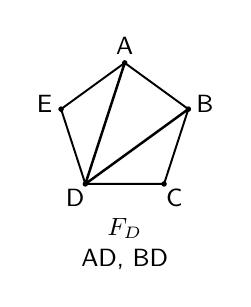
\begin{tikzpicture}[baseline=(current bounding box.center),every node/.style={font=\small}]
\coordinate (v0) at (0.0000,0.8500);
\coordinate (v1) at (0.8084,0.2627);
\coordinate (v2) at (0.4996,-0.6877);
\coordinate (v3) at (-0.4996,-0.6877);
\coordinate (v4) at (-0.8084,0.2627);
\draw[line width=.7pt] (v0)--(v1)--(v2)--(v3)--(v4)--cycle;
\draw[line width=.9pt](v0)--(v3);
\draw[line width=.9pt](v1)--(v3);
\fill (v0) circle (1pt);\node at (0.0000,1.0700) {A};
\fill (v1) circle (1pt);\node at (1.0176,0.3306) {B};
\fill (v2) circle (1pt);\node at (0.6289,-0.8656) {C};
\fill (v3) circle (1pt);\node at (-0.6289,-0.8656) {D};
\fill (v4) circle (1pt);\node at (-1.0176,0.3306) {E};
\node[align=center,font=\small] at (0,-1.450) {$F_D$\\AD, BD};
\end{tikzpicture} & 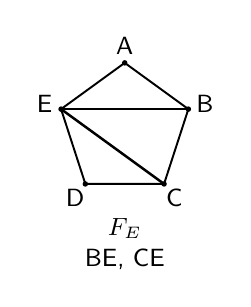
\begin{tikzpicture}[baseline=(current bounding box.center),every node/.style={font=\small}]
\coordinate (v0) at (0.0000,0.8500);
\coordinate (v1) at (0.8084,0.2627);
\coordinate (v2) at (0.4996,-0.6877);
\coordinate (v3) at (-0.4996,-0.6877);
\coordinate (v4) at (-0.8084,0.2627);
\draw[line width=.7pt] (v0)--(v1)--(v2)--(v3)--(v4)--cycle;
\draw[line width=.9pt](v1)--(v4);
\draw[line width=.9pt](v2)--(v4);
\fill (v0) circle (1pt);\node at (0.0000,1.0700) {A};
\fill (v1) circle (1pt);\node at (1.0176,0.3306) {B};
\fill (v2) circle (1pt);\node at (0.6289,-0.8656) {C};
\fill (v3) circle (1pt);\node at (-0.6289,-0.8656) {D};
\fill (v4) circle (1pt);\node at (-1.0176,0.3306) {E};
\node[align=center,font=\small] at (0,-1.450) {$F_E$\\BE, CE};
\end{tikzpicture}\\[7pt]
\end{tabular}\end{center}

\textbf{Why there are exactly five.} A pentagon filling uses two diagonals. If two pentagon diagonals have no common endpoint, their interiors cross, so the two legal diagonals share a corner. Both diagonals from that corner are then forced. Each of the five corners gives one distinct fan. This proves that the displayed list is complete. A second organizing method is to choose the triangle on a fixed boundary edge; the hexagon version appears on page 8.

\textbf{Why the triangle count stays fixed.} An $n$-corner polygon has $n-2$ triangles and $n-3$ diagonals in every triangulation. For induction, a triangle gives the base case. A diagonal divides an $n$-gon into polygons with $p$ and $q$ corners, where $p+q=n+2$. The smaller fillings contain $(p-2)+(q-2)=n-2$ triangles. They contain $(p-3)+(q-3)$ interior diagonals, plus the dividing diagonal, giving $n-3$. This argument uses a diagonal in an already complete filling; it does not prescribe how children must build one.

\textbf{Small counts for this packet}
\begin{center}\begin{tabular}{lrrrrrr}\toprule
Corners&3&4&5&6&7&8\\\midrule
Triangles in each filling&1&2&3&4&5&6\\
Diagonals in each filling&0&1&2&3&4&5\\
Different labeled fillings&1&2&5&14&42&132\\\bottomrule\end{tabular}\end{center}
The last row counts different whole fillings, not triangles inside one filling. Children need not enumerate the heptagon or octagon in this session.

\textbf{Common confusions.} A line between two neighboring corners is a boundary side, not a diagonal. A line through a new crossing point is illegal even if the pieces look triangular. A graph joining \emph{whole filling pictures} is a new kind of diagram; its joins are not diagonals inside the original polygon. Only the latter are subject to the noncrossing rule.

\newpage
\pagehead{K--1 solutions for Problems 1 to 4}
\prob{Problem 1}{Any two distinct legal fillings of each printed polygon suffice. For the pentagon, use $\{13,14\}$ and $\{24,25\}$. For the hexagon, use $\{13,14,15\}$ and $\{24,25,26\}$. Each pentagon has 3 triangles; each hexagon has 4.}
\hint{If a child repeats the same picture, compare the endpoints of every line. A tracing turned around without changing corner names is still the same filling.}
\prob{Problem 2}{There are five fillings, exactly the five fans on page 3 with letters replaced by numbers. Their diagonal sets are $\{13,14\}$, $\{24,25\}$, $\{13,35\}$, $\{14,24\}$, and $\{25,35\}$.}
\hint{Let the child keep each discovery on a separate tracing. When ready to check completeness, ask whether the two lines meet at a corner and which corner it is.}
\prob{Problem 3}{Three triangles are impossible; four are possible. For example, $\{13,14,15\}$ gives four. Any diagonal of a hexagon separates a triangle and a pentagon, or two quadrilaterals. Completing those sides gives $1+3=4$ or $2+2=4$ triangles. Thus changing the shape of the triangles cannot yield three.}
\hint{Ask the child to point to any uncovered region in a three-triangle attempt. For a child seeking a reason that covers every attempt, cover one side of a chosen diagonal and count the two smaller pieces separately.}
\prob{Problem 4}{Keeping 13 in the pentagon leaves a quadrilateral with two choices. Keeping 14 in the hexagon leaves two quadrilaterals, each with two independent choices: four completions. Here is the full answer collection.}
\begin{center}\begin{tabular}{cc}
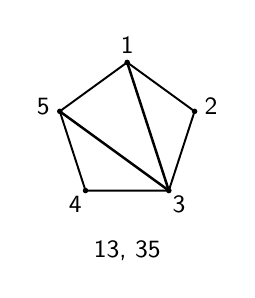
\begin{tikzpicture}[baseline=(current bounding box.center),every node/.style={font=\small}]
\coordinate (v0) at (0.0000,0.9000);
\coordinate (v1) at (0.8560,0.2781);
\coordinate (v2) at (0.5290,-0.7281);
\coordinate (v3) at (-0.5290,-0.7281);
\coordinate (v4) at (-0.8560,0.2781);
\draw[line width=.7pt] (v0)--(v1)--(v2)--(v3)--(v4)--cycle;
\draw[line width=.9pt](v0)--(v2);
\draw[line width=.9pt](v2)--(v4);
\fill (v0) circle (1pt);\node at (0.0000,1.1200) {1};
\fill (v1) circle (1pt);\node at (1.0652,0.3461) {2};
\fill (v2) circle (1pt);\node at (0.6583,-0.9061) {3};
\fill (v3) circle (1pt);\node at (-0.6583,-0.9061) {4};
\fill (v4) circle (1pt);\node at (-1.0652,0.3461) {5};
\node[align=center,font=\small] at (0,-1.500) {13, 35};
\end{tikzpicture} & 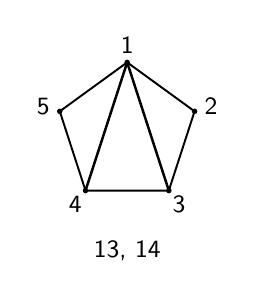
\begin{tikzpicture}[baseline=(current bounding box.center),every node/.style={font=\small}]
\coordinate (v0) at (0.0000,0.9000);
\coordinate (v1) at (0.8560,0.2781);
\coordinate (v2) at (0.5290,-0.7281);
\coordinate (v3) at (-0.5290,-0.7281);
\coordinate (v4) at (-0.8560,0.2781);
\draw[line width=.7pt] (v0)--(v1)--(v2)--(v3)--(v4)--cycle;
\draw[line width=.9pt](v0)--(v2);
\draw[line width=.9pt](v0)--(v3);
\fill (v0) circle (1pt);\node at (0.0000,1.1200) {1};
\fill (v1) circle (1pt);\node at (1.0652,0.3461) {2};
\fill (v2) circle (1pt);\node at (0.6583,-0.9061) {3};
\fill (v3) circle (1pt);\node at (-0.6583,-0.9061) {4};
\fill (v4) circle (1pt);\node at (-1.0652,0.3461) {5};
\node[align=center,font=\small] at (0,-1.500) {13, 14};
\end{tikzpicture}\\[7pt]
\end{tabular}\end{center}
\begin{center}\begin{tabular}{cccc}
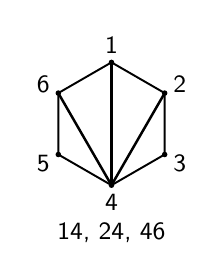
\begin{tikzpicture}[baseline=(current bounding box.center),every node/.style={font=\small}]
\coordinate (v0) at (0.0000,0.7800);
\coordinate (v1) at (0.6755,0.3900);
\coordinate (v2) at (0.6755,-0.3900);
\coordinate (v3) at (0.0000,-0.7800);
\coordinate (v4) at (-0.6755,-0.3900);
\coordinate (v5) at (-0.6755,0.3900);
\draw[line width=.7pt] (v0)--(v1)--(v2)--(v3)--(v4)--(v5)--cycle;
\draw[line width=.9pt](v0)--(v3);
\draw[line width=.9pt](v1)--(v3);
\draw[line width=.9pt](v3)--(v5);
\fill (v0) circle (1pt);\node at (0.0000,1.0000) {1};
\fill (v1) circle (1pt);\node at (0.8660,0.5000) {2};
\fill (v2) circle (1pt);\node at (0.8660,-0.5000) {3};
\fill (v3) circle (1pt);\node at (0.0000,-1.0000) {4};
\fill (v4) circle (1pt);\node at (-0.8660,-0.5000) {5};
\fill (v5) circle (1pt);\node at (-0.8660,0.5000) {6};
\node[align=center,font=\small] at (0,-1.380) {14, 24, 46};
\end{tikzpicture} & 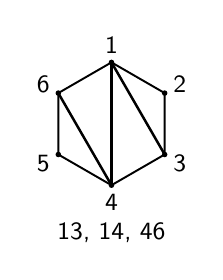
\begin{tikzpicture}[baseline=(current bounding box.center),every node/.style={font=\small}]
\coordinate (v0) at (0.0000,0.7800);
\coordinate (v1) at (0.6755,0.3900);
\coordinate (v2) at (0.6755,-0.3900);
\coordinate (v3) at (0.0000,-0.7800);
\coordinate (v4) at (-0.6755,-0.3900);
\coordinate (v5) at (-0.6755,0.3900);
\draw[line width=.7pt] (v0)--(v1)--(v2)--(v3)--(v4)--(v5)--cycle;
\draw[line width=.9pt](v0)--(v2);
\draw[line width=.9pt](v0)--(v3);
\draw[line width=.9pt](v3)--(v5);
\fill (v0) circle (1pt);\node at (0.0000,1.0000) {1};
\fill (v1) circle (1pt);\node at (0.8660,0.5000) {2};
\fill (v2) circle (1pt);\node at (0.8660,-0.5000) {3};
\fill (v3) circle (1pt);\node at (0.0000,-1.0000) {4};
\fill (v4) circle (1pt);\node at (-0.8660,-0.5000) {5};
\fill (v5) circle (1pt);\node at (-0.8660,0.5000) {6};
\node[align=center,font=\small] at (0,-1.380) {13, 14, 46};
\end{tikzpicture} & 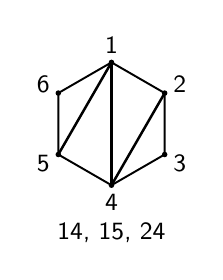
\begin{tikzpicture}[baseline=(current bounding box.center),every node/.style={font=\small}]
\coordinate (v0) at (0.0000,0.7800);
\coordinate (v1) at (0.6755,0.3900);
\coordinate (v2) at (0.6755,-0.3900);
\coordinate (v3) at (0.0000,-0.7800);
\coordinate (v4) at (-0.6755,-0.3900);
\coordinate (v5) at (-0.6755,0.3900);
\draw[line width=.7pt] (v0)--(v1)--(v2)--(v3)--(v4)--(v5)--cycle;
\draw[line width=.9pt](v0)--(v3);
\draw[line width=.9pt](v0)--(v4);
\draw[line width=.9pt](v1)--(v3);
\fill (v0) circle (1pt);\node at (0.0000,1.0000) {1};
\fill (v1) circle (1pt);\node at (0.8660,0.5000) {2};
\fill (v2) circle (1pt);\node at (0.8660,-0.5000) {3};
\fill (v3) circle (1pt);\node at (0.0000,-1.0000) {4};
\fill (v4) circle (1pt);\node at (-0.8660,-0.5000) {5};
\fill (v5) circle (1pt);\node at (-0.8660,0.5000) {6};
\node[align=center,font=\small] at (0,-1.380) {14, 15, 24};
\end{tikzpicture} & 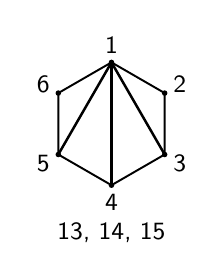
\begin{tikzpicture}[baseline=(current bounding box.center),every node/.style={font=\small}]
\coordinate (v0) at (0.0000,0.7800);
\coordinate (v1) at (0.6755,0.3900);
\coordinate (v2) at (0.6755,-0.3900);
\coordinate (v3) at (0.0000,-0.7800);
\coordinate (v4) at (-0.6755,-0.3900);
\coordinate (v5) at (-0.6755,0.3900);
\draw[line width=.7pt] (v0)--(v1)--(v2)--(v3)--(v4)--(v5)--cycle;
\draw[line width=.9pt](v0)--(v2);
\draw[line width=.9pt](v0)--(v3);
\draw[line width=.9pt](v0)--(v4);
\fill (v0) circle (1pt);\node at (0.0000,1.0000) {1};
\fill (v1) circle (1pt);\node at (0.8660,0.5000) {2};
\fill (v2) circle (1pt);\node at (0.8660,-0.5000) {3};
\fill (v3) circle (1pt);\node at (0.0000,-1.0000) {4};
\fill (v4) circle (1pt);\node at (-0.8660,-0.5000) {5};
\fill (v5) circle (1pt);\node at (-0.8660,0.5000) {6};
\node[align=center,font=\small] at (0,-1.380) {13, 14, 15};
\end{tikzpicture}\\[7pt]
\end{tabular}\end{center}
\hint{Keep the required printed diagonal visible on every tracing. If one hexagon side is always filled the same way, ask whether its quadrilateral has another filling. Combining each left choice with each right choice proves completeness.}

\newpage
\pagehead{K--1 solutions for Problems 5 and 6}
\prob{Problem 5}{Each printed hexagon has exactly three one-change results, one for each of its three interior diagonals. The original filling itself is not a new result.}
\textbf{First start} $\{13,14,15\}$ has these three neighbors:
\begin{center}\begin{tabular}{ccc}
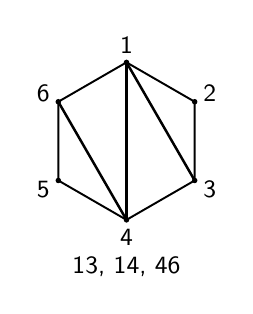
\begin{tikzpicture}[baseline=(current bounding box.center),every node/.style={font=\small}]
\coordinate (v0) at (0.0000,1.0000);
\coordinate (v1) at (0.8660,0.5000);
\coordinate (v2) at (0.8660,-0.5000);
\coordinate (v3) at (0.0000,-1.0000);
\coordinate (v4) at (-0.8660,-0.5000);
\coordinate (v5) at (-0.8660,0.5000);
\draw[line width=.7pt] (v0)--(v1)--(v2)--(v3)--(v4)--(v5)--cycle;
\draw[line width=.9pt](v0)--(v2);
\draw[line width=.9pt](v0)--(v3);
\draw[line width=.9pt](v3)--(v5);
\fill (v0) circle (1pt);\node at (0.0000,1.2200) {1};
\fill (v1) circle (1pt);\node at (1.0566,0.6100) {2};
\fill (v2) circle (1pt);\node at (1.0566,-0.6100) {3};
\fill (v3) circle (1pt);\node at (0.0000,-1.2200) {4};
\fill (v4) circle (1pt);\node at (-1.0566,-0.6100) {5};
\fill (v5) circle (1pt);\node at (-1.0566,0.6100) {6};
\node[align=center,font=\small] at (0,-1.600) {13, 14, 46};
\end{tikzpicture} & 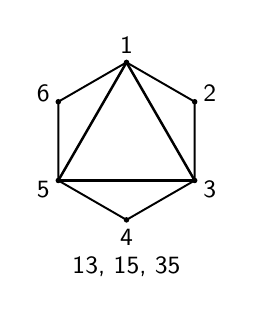
\begin{tikzpicture}[baseline=(current bounding box.center),every node/.style={font=\small}]
\coordinate (v0) at (0.0000,1.0000);
\coordinate (v1) at (0.8660,0.5000);
\coordinate (v2) at (0.8660,-0.5000);
\coordinate (v3) at (0.0000,-1.0000);
\coordinate (v4) at (-0.8660,-0.5000);
\coordinate (v5) at (-0.8660,0.5000);
\draw[line width=.7pt] (v0)--(v1)--(v2)--(v3)--(v4)--(v5)--cycle;
\draw[line width=.9pt](v0)--(v2);
\draw[line width=.9pt](v0)--(v4);
\draw[line width=.9pt](v2)--(v4);
\fill (v0) circle (1pt);\node at (0.0000,1.2200) {1};
\fill (v1) circle (1pt);\node at (1.0566,0.6100) {2};
\fill (v2) circle (1pt);\node at (1.0566,-0.6100) {3};
\fill (v3) circle (1pt);\node at (0.0000,-1.2200) {4};
\fill (v4) circle (1pt);\node at (-1.0566,-0.6100) {5};
\fill (v5) circle (1pt);\node at (-1.0566,0.6100) {6};
\node[align=center,font=\small] at (0,-1.600) {13, 15, 35};
\end{tikzpicture} & 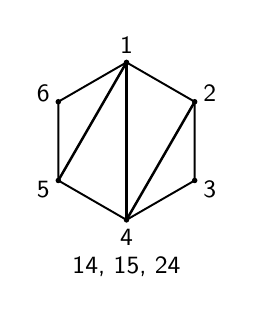
\begin{tikzpicture}[baseline=(current bounding box.center),every node/.style={font=\small}]
\coordinate (v0) at (0.0000,1.0000);
\coordinate (v1) at (0.8660,0.5000);
\coordinate (v2) at (0.8660,-0.5000);
\coordinate (v3) at (0.0000,-1.0000);
\coordinate (v4) at (-0.8660,-0.5000);
\coordinate (v5) at (-0.8660,0.5000);
\draw[line width=.7pt] (v0)--(v1)--(v2)--(v3)--(v4)--(v5)--cycle;
\draw[line width=.9pt](v0)--(v3);
\draw[line width=.9pt](v0)--(v4);
\draw[line width=.9pt](v1)--(v3);
\fill (v0) circle (1pt);\node at (0.0000,1.2200) {1};
\fill (v1) circle (1pt);\node at (1.0566,0.6100) {2};
\fill (v2) circle (1pt);\node at (1.0566,-0.6100) {3};
\fill (v3) circle (1pt);\node at (0.0000,-1.2200) {4};
\fill (v4) circle (1pt);\node at (-1.0566,-0.6100) {5};
\fill (v5) circle (1pt);\node at (-1.0566,0.6100) {6};
\node[align=center,font=\small] at (0,-1.600) {14, 15, 24};
\end{tikzpicture}\\[7pt]
\end{tabular}\end{center}
\textbf{Second start} $\{13,15,35\}$ has these three neighbors:
\begin{center}\begin{tabular}{ccc}
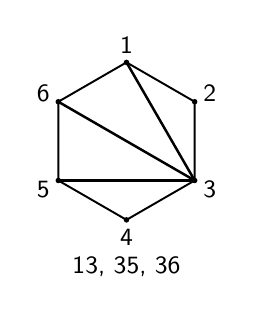
\begin{tikzpicture}[baseline=(current bounding box.center),every node/.style={font=\small}]
\coordinate (v0) at (0.0000,1.0000);
\coordinate (v1) at (0.8660,0.5000);
\coordinate (v2) at (0.8660,-0.5000);
\coordinate (v3) at (0.0000,-1.0000);
\coordinate (v4) at (-0.8660,-0.5000);
\coordinate (v5) at (-0.8660,0.5000);
\draw[line width=.7pt] (v0)--(v1)--(v2)--(v3)--(v4)--(v5)--cycle;
\draw[line width=.9pt](v0)--(v2);
\draw[line width=.9pt](v2)--(v4);
\draw[line width=.9pt](v2)--(v5);
\fill (v0) circle (1pt);\node at (0.0000,1.2200) {1};
\fill (v1) circle (1pt);\node at (1.0566,0.6100) {2};
\fill (v2) circle (1pt);\node at (1.0566,-0.6100) {3};
\fill (v3) circle (1pt);\node at (0.0000,-1.2200) {4};
\fill (v4) circle (1pt);\node at (-1.0566,-0.6100) {5};
\fill (v5) circle (1pt);\node at (-1.0566,0.6100) {6};
\node[align=center,font=\small] at (0,-1.600) {13, 35, 36};
\end{tikzpicture} & 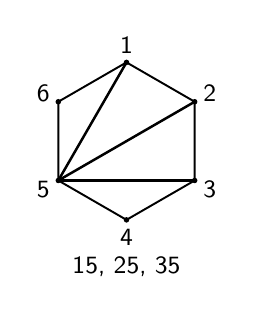
\begin{tikzpicture}[baseline=(current bounding box.center),every node/.style={font=\small}]
\coordinate (v0) at (0.0000,1.0000);
\coordinate (v1) at (0.8660,0.5000);
\coordinate (v2) at (0.8660,-0.5000);
\coordinate (v3) at (0.0000,-1.0000);
\coordinate (v4) at (-0.8660,-0.5000);
\coordinate (v5) at (-0.8660,0.5000);
\draw[line width=.7pt] (v0)--(v1)--(v2)--(v3)--(v4)--(v5)--cycle;
\draw[line width=.9pt](v0)--(v4);
\draw[line width=.9pt](v1)--(v4);
\draw[line width=.9pt](v2)--(v4);
\fill (v0) circle (1pt);\node at (0.0000,1.2200) {1};
\fill (v1) circle (1pt);\node at (1.0566,0.6100) {2};
\fill (v2) circle (1pt);\node at (1.0566,-0.6100) {3};
\fill (v3) circle (1pt);\node at (0.0000,-1.2200) {4};
\fill (v4) circle (1pt);\node at (-1.0566,-0.6100) {5};
\fill (v5) circle (1pt);\node at (-1.0566,0.6100) {6};
\node[align=center,font=\small] at (0,-1.600) {15, 25, 35};
\end{tikzpicture} & 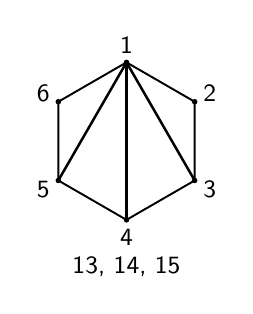
\begin{tikzpicture}[baseline=(current bounding box.center),every node/.style={font=\small}]
\coordinate (v0) at (0.0000,1.0000);
\coordinate (v1) at (0.8660,0.5000);
\coordinate (v2) at (0.8660,-0.5000);
\coordinate (v3) at (0.0000,-1.0000);
\coordinate (v4) at (-0.8660,-0.5000);
\coordinate (v5) at (-0.8660,0.5000);
\draw[line width=.7pt] (v0)--(v1)--(v2)--(v3)--(v4)--(v5)--cycle;
\draw[line width=.9pt](v0)--(v2);
\draw[line width=.9pt](v0)--(v3);
\draw[line width=.9pt](v0)--(v4);
\fill (v0) circle (1pt);\node at (0.0000,1.2200) {1};
\fill (v1) circle (1pt);\node at (1.0566,0.6100) {2};
\fill (v2) circle (1pt);\node at (1.0566,-0.6100) {3};
\fill (v3) circle (1pt);\node at (0.0000,-1.2200) {4};
\fill (v4) circle (1pt);\node at (-1.0566,-0.6100) {5};
\fill (v5) circle (1pt);\node at (-1.0566,0.6100) {6};
\node[align=center,font=\small] at (0,-1.600) {13, 14, 15};
\end{tikzpicture}\\[7pt]
\end{tabular}\end{center}

\textbf{Why the list is complete.} Removing one interior diagonal merges exactly its two adjacent triangles into a convex quadrilateral. That quadrilateral has exactly one other diagonal. Everything outside it is unchanged. Thus each of the three original diagonals supplies exactly one neighbor, and there are no further legal one-line replacements.
\hint{Trace the two triangles touching the line a child wants to erase. Ask for the boundary of their combined piece before asking which other line fills it. Do not erase a second line.}
\prob{Problem 6}{Yes. Name a pentagon filling by the corner where its two diagonals meet. The route $1,3,5,2,4,1$ visits every other filling once and returns in five changes. The route in the opposite direction works too. Its complete diagonal sets are}
\[
\{13,14\}\to\{13,35\}\to\{25,35\}\to
\{24,25\}\to\{14,24\}\to\{13,14\}.
\]
Each arrow replaces exactly one line. The pentagon map on page 6 shows why all five fillings have been visited.
\hint{Lay the five earlier tracings around the table. Ask which ones can follow the current picture after one change. Keep the used tracings separate until it is time to return.}
\textbf{Useful stopping point.} Children who build and explain this five-step loop have encountered a genuine odd cycle. They do not need the word ``parity'' or the older packet's distance formula.

\newpage
\pagehead{Grades 2--3 solutions for Problems 1 to 5}
\prob{Problem 1}{Any two distinct legal fillings suffice. Hexagon examples: $\{AC,AD,AE\}$ and $\{BD,BE,BF\}$. Heptagon examples: $\{AC,AD,AE,AF\}$ and $\{BD,BE,BF,BG\}$. The counts cannot differ: every hexagon filling has 4 triangles and every heptagon filling has 5. Use page 3's splitting argument if children seek an explanation.}
\hint{Ask whether a thin or large triangle should still count as one. The task uses all triangles, regardless of size or shape.}
\prob{Problem 2}{Exactly five pentagon fillings, displayed on page 3. The shared-corner argument there proves completeness.}
\hint{Sort a child's collection by the corner shared by its two diagonals. Keep corner names fixed so that all five fans remain distinct.}
\prob{Problem 3}{First start $\{AC,AD,AE\}$ has neighbors $\{AC,AD,DF\}$, $\{AC,AE,CE\}$, and $\{AD,AE,BD\}$. Second start $\{AC,AE,CE\}$ has neighbors $\{AC,CE,CF\}$, $\{AE,BE,CE\}$, and $\{AC,AD,AE\}$. The six diagrams on page 5 show all results after replacing number labels by letters.}
\hint{Choose one original diagonal; identify its two incident triangles. The other diagonal of their quadrilateral is the only legal replacement.}
\prob{Problem 4}{The complete pentagon map has exactly five joins: $F_A F_C$, $F_C F_E$, $F_E F_B$, $F_B F_D$, $F_D F_A$. There are no other joins. The revised student layout follows this cycle around the page.}
\begin{center}
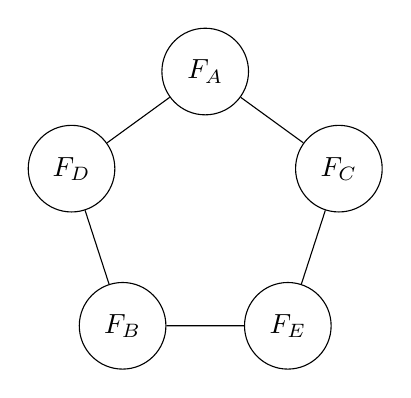
\begin{tikzpicture}[>=Stealth,every node/.style={draw,circle,minimum size=11mm},scale=.85]
\foreach \name/\angle in {A/90,C/18,E/-54,B/-126,D/162}{\node(\name) at (\angle:2.1) {$F_{\name}$};}
\draw(A)--(C)--(E)--(B)--(D)--(A);
\end{tikzpicture}
\end{center}
Each adjacent pair keeps one diagonal and replaces the other. Each of the five fillings has only two interior diagonals, hence exactly two possible flips; the displayed joins account for both and prove completeness.
\prob{Problem 5}{An odd return route is $F_A,F_C,F_E,F_B,F_D,F_A$, with five flips. The complete sets are the K--1 P6 route with letters replacing numbers. No shorter odd return is possible: this graph has no loops or triangles. An immediate out-and-back takes two flips and does not meet the odd condition.}
\hint{Ask children to trace the joins with a finger and count \emph{moves}, not pictures. Six listed pictures represent five flips when the first is repeated at the end.}

\newpage
\pagehead{Grades 2--3 Problem 6 and shortest routes}
\prob{Problem 6}{The printed start is the B fan $\{BD,BE,BF\}$ and the target is the A fan $\{AC,AD,AE\}$. The minimum is three flips. Here is one shortest route, read left to right:}
\begin{center}\begin{tabular}{cccc}
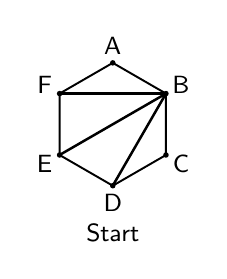
\begin{tikzpicture}[baseline=(current bounding box.center),every node/.style={font=\small}]
\coordinate (v0) at (0.0000,0.7800);
\coordinate (v1) at (0.6755,0.3900);
\coordinate (v2) at (0.6755,-0.3900);
\coordinate (v3) at (0.0000,-0.7800);
\coordinate (v4) at (-0.6755,-0.3900);
\coordinate (v5) at (-0.6755,0.3900);
\draw[line width=.7pt] (v0)--(v1)--(v2)--(v3)--(v4)--(v5)--cycle;
\draw[line width=.9pt](v1)--(v3);
\draw[line width=.9pt](v1)--(v4);
\draw[line width=.9pt](v1)--(v5);
\fill (v0) circle (1pt);\node at (0.0000,1.0000) {A};
\fill (v1) circle (1pt);\node at (0.8660,0.5000) {B};
\fill (v2) circle (1pt);\node at (0.8660,-0.5000) {C};
\fill (v3) circle (1pt);\node at (0.0000,-1.0000) {D};
\fill (v4) circle (1pt);\node at (-0.8660,-0.5000) {E};
\fill (v5) circle (1pt);\node at (-0.8660,0.5000) {F};
\node[align=center,font=\small] at (0,-1.380) {Start};
\end{tikzpicture} & 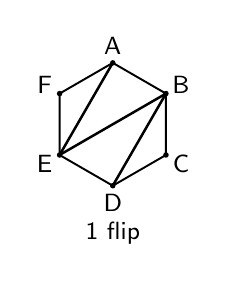
\begin{tikzpicture}[baseline=(current bounding box.center),every node/.style={font=\small}]
\coordinate (v0) at (0.0000,0.7800);
\coordinate (v1) at (0.6755,0.3900);
\coordinate (v2) at (0.6755,-0.3900);
\coordinate (v3) at (0.0000,-0.7800);
\coordinate (v4) at (-0.6755,-0.3900);
\coordinate (v5) at (-0.6755,0.3900);
\draw[line width=.7pt] (v0)--(v1)--(v2)--(v3)--(v4)--(v5)--cycle;
\draw[line width=.9pt](v0)--(v4);
\draw[line width=.9pt](v1)--(v3);
\draw[line width=.9pt](v1)--(v4);
\fill (v0) circle (1pt);\node at (0.0000,1.0000) {A};
\fill (v1) circle (1pt);\node at (0.8660,0.5000) {B};
\fill (v2) circle (1pt);\node at (0.8660,-0.5000) {C};
\fill (v3) circle (1pt);\node at (0.0000,-1.0000) {D};
\fill (v4) circle (1pt);\node at (-0.8660,-0.5000) {E};
\fill (v5) circle (1pt);\node at (-0.8660,0.5000) {F};
\node[align=center,font=\small] at (0,-1.380) {1 flip};
\end{tikzpicture} & 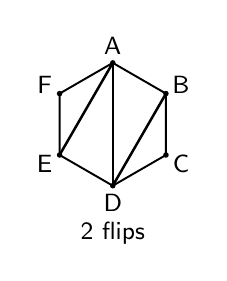
\begin{tikzpicture}[baseline=(current bounding box.center),every node/.style={font=\small}]
\coordinate (v0) at (0.0000,0.7800);
\coordinate (v1) at (0.6755,0.3900);
\coordinate (v2) at (0.6755,-0.3900);
\coordinate (v3) at (0.0000,-0.7800);
\coordinate (v4) at (-0.6755,-0.3900);
\coordinate (v5) at (-0.6755,0.3900);
\draw[line width=.7pt] (v0)--(v1)--(v2)--(v3)--(v4)--(v5)--cycle;
\draw[line width=.9pt](v0)--(v3);
\draw[line width=.9pt](v0)--(v4);
\draw[line width=.9pt](v1)--(v3);
\fill (v0) circle (1pt);\node at (0.0000,1.0000) {A};
\fill (v1) circle (1pt);\node at (0.8660,0.5000) {B};
\fill (v2) circle (1pt);\node at (0.8660,-0.5000) {C};
\fill (v3) circle (1pt);\node at (0.0000,-1.0000) {D};
\fill (v4) circle (1pt);\node at (-0.8660,-0.5000) {E};
\fill (v5) circle (1pt);\node at (-0.8660,0.5000) {F};
\node[align=center,font=\small] at (0,-1.380) {2 flips};
\end{tikzpicture} & 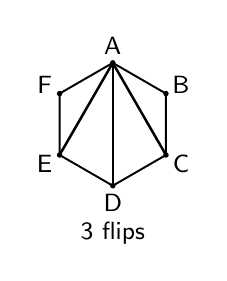
\begin{tikzpicture}[baseline=(current bounding box.center),every node/.style={font=\small}]
\coordinate (v0) at (0.0000,0.7800);
\coordinate (v1) at (0.6755,0.3900);
\coordinate (v2) at (0.6755,-0.3900);
\coordinate (v3) at (0.0000,-0.7800);
\coordinate (v4) at (-0.6755,-0.3900);
\coordinate (v5) at (-0.6755,0.3900);
\draw[line width=.7pt] (v0)--(v1)--(v2)--(v3)--(v4)--(v5)--cycle;
\draw[line width=.9pt](v0)--(v2);
\draw[line width=.9pt](v0)--(v3);
\draw[line width=.9pt](v0)--(v4);
\fill (v0) circle (1pt);\node at (0.0000,1.0000) {A};
\fill (v1) circle (1pt);\node at (0.8660,0.5000) {B};
\fill (v2) circle (1pt);\node at (0.8660,-0.5000) {C};
\fill (v3) circle (1pt);\node at (0.0000,-1.0000) {D};
\fill (v4) circle (1pt);\node at (-0.8660,-0.5000) {E};
\fill (v5) circle (1pt);\node at (-0.8660,0.5000) {F};
\node[align=center,font=\small] at (0,-1.380) {3 flips};
\end{tikzpicture}\\[7pt]
\end{tabular}\end{center}
\begin{center}\begin{tabular}{rll}\toprule Step & Diagonals in the filling & Change just made\\\midrule
0 & BD, BE, BF & Start\\
1 & AE, BD, BE & BF $\to$ AE\\
2 & AD, AE, BD & BE $\to$ AD\\
3 & AC, AD, AE & BD $\to$ AC\\
\bottomrule\end{tabular}\end{center}

\textbf{Why three is best.} None of the three target diagonals is present initially. One flip adds only one diagonal, so at least three flips are necessary. The displayed route achieves three. Counting missing target diagonals is a lower bound for arbitrary targets; it is always attainable for a fan target (page 11).

\textbf{A different simple route has four flips.} The following five pictures are all different, so this meets the revised requirement to avoid visiting a filling twice.
\begin{center}\begin{tabular}{ccccc}
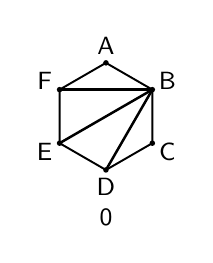
\begin{tikzpicture}[baseline=(current bounding box.center),every node/.style={font=\small}]
\coordinate (v0) at (0.0000,0.6800);
\coordinate (v1) at (0.5889,0.3400);
\coordinate (v2) at (0.5889,-0.3400);
\coordinate (v3) at (0.0000,-0.6800);
\coordinate (v4) at (-0.5889,-0.3400);
\coordinate (v5) at (-0.5889,0.3400);
\draw[line width=.7pt] (v0)--(v1)--(v2)--(v3)--(v4)--(v5)--cycle;
\draw[line width=.9pt](v1)--(v3);
\draw[line width=.9pt](v1)--(v4);
\draw[line width=.9pt](v1)--(v5);
\fill (v0) circle (1pt);\node at (0.0000,0.9000) {A};
\fill (v1) circle (1pt);\node at (0.7794,0.4500) {B};
\fill (v2) circle (1pt);\node at (0.7794,-0.4500) {C};
\fill (v3) circle (1pt);\node at (0.0000,-0.9000) {D};
\fill (v4) circle (1pt);\node at (-0.7794,-0.4500) {E};
\fill (v5) circle (1pt);\node at (-0.7794,0.4500) {F};
\node[align=center,font=\small] at (0,-1.280) {0};
\end{tikzpicture} & 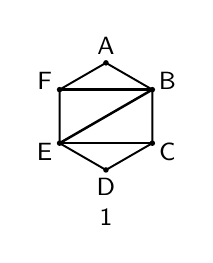
\begin{tikzpicture}[baseline=(current bounding box.center),every node/.style={font=\small}]
\coordinate (v0) at (0.0000,0.6800);
\coordinate (v1) at (0.5889,0.3400);
\coordinate (v2) at (0.5889,-0.3400);
\coordinate (v3) at (0.0000,-0.6800);
\coordinate (v4) at (-0.5889,-0.3400);
\coordinate (v5) at (-0.5889,0.3400);
\draw[line width=.7pt] (v0)--(v1)--(v2)--(v3)--(v4)--(v5)--cycle;
\draw[line width=.9pt](v1)--(v4);
\draw[line width=.9pt](v1)--(v5);
\draw[line width=.9pt](v2)--(v4);
\fill (v0) circle (1pt);\node at (0.0000,0.9000) {A};
\fill (v1) circle (1pt);\node at (0.7794,0.4500) {B};
\fill (v2) circle (1pt);\node at (0.7794,-0.4500) {C};
\fill (v3) circle (1pt);\node at (0.0000,-0.9000) {D};
\fill (v4) circle (1pt);\node at (-0.7794,-0.4500) {E};
\fill (v5) circle (1pt);\node at (-0.7794,0.4500) {F};
\node[align=center,font=\small] at (0,-1.280) {1};
\end{tikzpicture} & 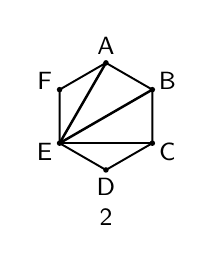
\begin{tikzpicture}[baseline=(current bounding box.center),every node/.style={font=\small}]
\coordinate (v0) at (0.0000,0.6800);
\coordinate (v1) at (0.5889,0.3400);
\coordinate (v2) at (0.5889,-0.3400);
\coordinate (v3) at (0.0000,-0.6800);
\coordinate (v4) at (-0.5889,-0.3400);
\coordinate (v5) at (-0.5889,0.3400);
\draw[line width=.7pt] (v0)--(v1)--(v2)--(v3)--(v4)--(v5)--cycle;
\draw[line width=.9pt](v0)--(v4);
\draw[line width=.9pt](v1)--(v4);
\draw[line width=.9pt](v2)--(v4);
\fill (v0) circle (1pt);\node at (0.0000,0.9000) {A};
\fill (v1) circle (1pt);\node at (0.7794,0.4500) {B};
\fill (v2) circle (1pt);\node at (0.7794,-0.4500) {C};
\fill (v3) circle (1pt);\node at (0.0000,-0.9000) {D};
\fill (v4) circle (1pt);\node at (-0.7794,-0.4500) {E};
\fill (v5) circle (1pt);\node at (-0.7794,0.4500) {F};
\node[align=center,font=\small] at (0,-1.280) {2};
\end{tikzpicture} & 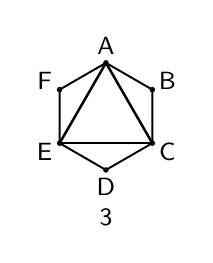
\begin{tikzpicture}[baseline=(current bounding box.center),every node/.style={font=\small}]
\coordinate (v0) at (0.0000,0.6800);
\coordinate (v1) at (0.5889,0.3400);
\coordinate (v2) at (0.5889,-0.3400);
\coordinate (v3) at (0.0000,-0.6800);
\coordinate (v4) at (-0.5889,-0.3400);
\coordinate (v5) at (-0.5889,0.3400);
\draw[line width=.7pt] (v0)--(v1)--(v2)--(v3)--(v4)--(v5)--cycle;
\draw[line width=.9pt](v0)--(v2);
\draw[line width=.9pt](v0)--(v4);
\draw[line width=.9pt](v2)--(v4);
\fill (v0) circle (1pt);\node at (0.0000,0.9000) {A};
\fill (v1) circle (1pt);\node at (0.7794,0.4500) {B};
\fill (v2) circle (1pt);\node at (0.7794,-0.4500) {C};
\fill (v3) circle (1pt);\node at (0.0000,-0.9000) {D};
\fill (v4) circle (1pt);\node at (-0.7794,-0.4500) {E};
\fill (v5) circle (1pt);\node at (-0.7794,0.4500) {F};
\node[align=center,font=\small] at (0,-1.280) {3};
\end{tikzpicture} & 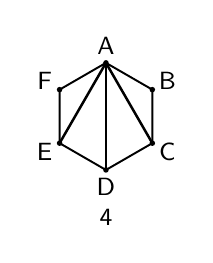
\begin{tikzpicture}[baseline=(current bounding box.center),every node/.style={font=\small}]
\coordinate (v0) at (0.0000,0.6800);
\coordinate (v1) at (0.5889,0.3400);
\coordinate (v2) at (0.5889,-0.3400);
\coordinate (v3) at (0.0000,-0.6800);
\coordinate (v4) at (-0.5889,-0.3400);
\coordinate (v5) at (-0.5889,0.3400);
\draw[line width=.7pt] (v0)--(v1)--(v2)--(v3)--(v4)--(v5)--cycle;
\draw[line width=.9pt](v0)--(v2);
\draw[line width=.9pt](v0)--(v3);
\draw[line width=.9pt](v0)--(v4);
\fill (v0) circle (1pt);\node at (0.0000,0.9000) {A};
\fill (v1) circle (1pt);\node at (0.7794,0.4500) {B};
\fill (v2) circle (1pt);\node at (0.7794,-0.4500) {C};
\fill (v3) circle (1pt);\node at (0.0000,-0.9000) {D};
\fill (v4) circle (1pt);\node at (-0.7794,-0.4500) {E};
\fill (v5) circle (1pt);\node at (-0.7794,0.4500) {F};
\node[align=center,font=\small] at (0,-1.280) {4};
\end{tikzpicture}\\[7pt]
\end{tabular}\end{center}
\begin{center}\begin{tabular}{rll}\toprule Step & Diagonals in the filling & Change just made\\\midrule
0 & BD, BE, BF & Start\\
1 & BE, BF, CE & BD $\to$ CE\\
2 & AE, BE, CE & BF $\to$ AE\\
3 & AC, AE, CE & BE $\to$ AC\\
4 & AC, AD, AE & CE $\to$ AD\\
\bottomrule\end{tabular}\end{center}

\hint{For the shortest route, ask which target lines are missing and how many can appear in one move. For the second route, try a different first move. Undoing and redoing a move does not satisfy the no-repeated-fillings instruction.}
\textbf{Check the actual move.} Two diagonal lists of length three are flip neighbors when they share exactly two diagonals. Merely rotating a page is not a move; nor may the child replace two diagonals at once.

\newpage
\pagehead{Grades 2--3 Problem 7 and all fourteen fillings}
\prob{Problem 7}{Student page 8 is labeled ``Problem 7 (continued): Extra hexagons for your collection.'' It supplies recording space for the same problem, not a second task. The complete hexagon collection has 14 fillings. The catalog below is organized by the triangle touching boundary edge AF. Its third corner is B, C, D, or E.}
\textbf{Third corner B: five fillings.} Diagonal BF cuts off triangle ABF, leaving a pentagon with five choices.
\begin{center}\begin{tabular}{ccccc}
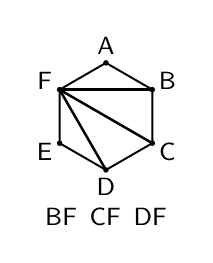
\begin{tikzpicture}[baseline=(current bounding box.center),every node/.style={font=\small}]
\coordinate (v0) at (0.0000,0.6800);
\coordinate (v1) at (0.5889,0.3400);
\coordinate (v2) at (0.5889,-0.3400);
\coordinate (v3) at (0.0000,-0.6800);
\coordinate (v4) at (-0.5889,-0.3400);
\coordinate (v5) at (-0.5889,0.3400);
\draw[line width=.7pt] (v0)--(v1)--(v2)--(v3)--(v4)--(v5)--cycle;
\draw[line width=.9pt](v1)--(v5);
\draw[line width=.9pt](v2)--(v5);
\draw[line width=.9pt](v3)--(v5);
\fill (v0) circle (1pt);\node at (0.0000,0.9000) {A};
\fill (v1) circle (1pt);\node at (0.7794,0.4500) {B};
\fill (v2) circle (1pt);\node at (0.7794,-0.4500) {C};
\fill (v3) circle (1pt);\node at (0.0000,-0.9000) {D};
\fill (v4) circle (1pt);\node at (-0.7794,-0.4500) {E};
\fill (v5) circle (1pt);\node at (-0.7794,0.4500) {F};
\node[align=center,font=\small] at (0,-1.280) {BF\, CF\, DF};
\end{tikzpicture} & 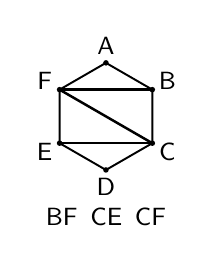
\begin{tikzpicture}[baseline=(current bounding box.center),every node/.style={font=\small}]
\coordinate (v0) at (0.0000,0.6800);
\coordinate (v1) at (0.5889,0.3400);
\coordinate (v2) at (0.5889,-0.3400);
\coordinate (v3) at (0.0000,-0.6800);
\coordinate (v4) at (-0.5889,-0.3400);
\coordinate (v5) at (-0.5889,0.3400);
\draw[line width=.7pt] (v0)--(v1)--(v2)--(v3)--(v4)--(v5)--cycle;
\draw[line width=.9pt](v1)--(v5);
\draw[line width=.9pt](v2)--(v4);
\draw[line width=.9pt](v2)--(v5);
\fill (v0) circle (1pt);\node at (0.0000,0.9000) {A};
\fill (v1) circle (1pt);\node at (0.7794,0.4500) {B};
\fill (v2) circle (1pt);\node at (0.7794,-0.4500) {C};
\fill (v3) circle (1pt);\node at (0.0000,-0.9000) {D};
\fill (v4) circle (1pt);\node at (-0.7794,-0.4500) {E};
\fill (v5) circle (1pt);\node at (-0.7794,0.4500) {F};
\node[align=center,font=\small] at (0,-1.280) {BF\, CE\, CF};
\end{tikzpicture} & 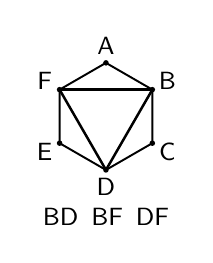
\begin{tikzpicture}[baseline=(current bounding box.center),every node/.style={font=\small}]
\coordinate (v0) at (0.0000,0.6800);
\coordinate (v1) at (0.5889,0.3400);
\coordinate (v2) at (0.5889,-0.3400);
\coordinate (v3) at (0.0000,-0.6800);
\coordinate (v4) at (-0.5889,-0.3400);
\coordinate (v5) at (-0.5889,0.3400);
\draw[line width=.7pt] (v0)--(v1)--(v2)--(v3)--(v4)--(v5)--cycle;
\draw[line width=.9pt](v1)--(v3);
\draw[line width=.9pt](v1)--(v5);
\draw[line width=.9pt](v3)--(v5);
\fill (v0) circle (1pt);\node at (0.0000,0.9000) {A};
\fill (v1) circle (1pt);\node at (0.7794,0.4500) {B};
\fill (v2) circle (1pt);\node at (0.7794,-0.4500) {C};
\fill (v3) circle (1pt);\node at (0.0000,-0.9000) {D};
\fill (v4) circle (1pt);\node at (-0.7794,-0.4500) {E};
\fill (v5) circle (1pt);\node at (-0.7794,0.4500) {F};
\node[align=center,font=\small] at (0,-1.280) {BD\, BF\, DF};
\end{tikzpicture} & 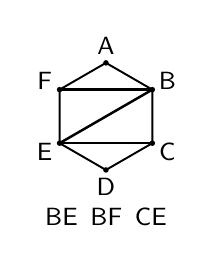
\begin{tikzpicture}[baseline=(current bounding box.center),every node/.style={font=\small}]
\coordinate (v0) at (0.0000,0.6800);
\coordinate (v1) at (0.5889,0.3400);
\coordinate (v2) at (0.5889,-0.3400);
\coordinate (v3) at (0.0000,-0.6800);
\coordinate (v4) at (-0.5889,-0.3400);
\coordinate (v5) at (-0.5889,0.3400);
\draw[line width=.7pt] (v0)--(v1)--(v2)--(v3)--(v4)--(v5)--cycle;
\draw[line width=.9pt](v1)--(v4);
\draw[line width=.9pt](v1)--(v5);
\draw[line width=.9pt](v2)--(v4);
\fill (v0) circle (1pt);\node at (0.0000,0.9000) {A};
\fill (v1) circle (1pt);\node at (0.7794,0.4500) {B};
\fill (v2) circle (1pt);\node at (0.7794,-0.4500) {C};
\fill (v3) circle (1pt);\node at (0.0000,-0.9000) {D};
\fill (v4) circle (1pt);\node at (-0.7794,-0.4500) {E};
\fill (v5) circle (1pt);\node at (-0.7794,0.4500) {F};
\node[align=center,font=\small] at (0,-1.280) {BE\, BF\, CE};
\end{tikzpicture} & 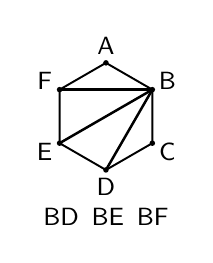
\begin{tikzpicture}[baseline=(current bounding box.center),every node/.style={font=\small}]
\coordinate (v0) at (0.0000,0.6800);
\coordinate (v1) at (0.5889,0.3400);
\coordinate (v2) at (0.5889,-0.3400);
\coordinate (v3) at (0.0000,-0.6800);
\coordinate (v4) at (-0.5889,-0.3400);
\coordinate (v5) at (-0.5889,0.3400);
\draw[line width=.7pt] (v0)--(v1)--(v2)--(v3)--(v4)--(v5)--cycle;
\draw[line width=.9pt](v1)--(v3);
\draw[line width=.9pt](v1)--(v4);
\draw[line width=.9pt](v1)--(v5);
\fill (v0) circle (1pt);\node at (0.0000,0.9000) {A};
\fill (v1) circle (1pt);\node at (0.7794,0.4500) {B};
\fill (v2) circle (1pt);\node at (0.7794,-0.4500) {C};
\fill (v3) circle (1pt);\node at (0.0000,-0.9000) {D};
\fill (v4) circle (1pt);\node at (-0.7794,-0.4500) {E};
\fill (v5) circle (1pt);\node at (-0.7794,0.4500) {F};
\node[align=center,font=\small] at (0,-1.280) {BD\, BE\, BF};
\end{tikzpicture}\\[7pt]
\end{tabular}\end{center}
\textbf{Third corner C: two fillings.} Triangle ACF leaves triangle ABC and quadrilateral CDEF.
\begin{center}\begin{tabular}{cc}
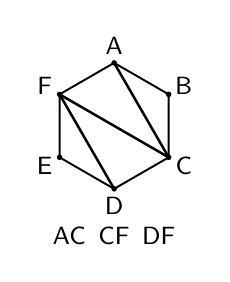
\begin{tikzpicture}[baseline=(current bounding box.center),every node/.style={font=\small}]
\coordinate (v0) at (0.0000,0.8000);
\coordinate (v1) at (0.6928,0.4000);
\coordinate (v2) at (0.6928,-0.4000);
\coordinate (v3) at (0.0000,-0.8000);
\coordinate (v4) at (-0.6928,-0.4000);
\coordinate (v5) at (-0.6928,0.4000);
\draw[line width=.7pt] (v0)--(v1)--(v2)--(v3)--(v4)--(v5)--cycle;
\draw[line width=.9pt](v0)--(v2);
\draw[line width=.9pt](v2)--(v5);
\draw[line width=.9pt](v3)--(v5);
\fill (v0) circle (1pt);\node at (0.0000,1.0200) {A};
\fill (v1) circle (1pt);\node at (0.8833,0.5100) {B};
\fill (v2) circle (1pt);\node at (0.8833,-0.5100) {C};
\fill (v3) circle (1pt);\node at (0.0000,-1.0200) {D};
\fill (v4) circle (1pt);\node at (-0.8833,-0.5100) {E};
\fill (v5) circle (1pt);\node at (-0.8833,0.5100) {F};
\node[align=center,font=\small] at (0,-1.400) {AC\, CF\, DF};
\end{tikzpicture} & 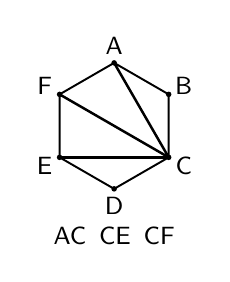
\begin{tikzpicture}[baseline=(current bounding box.center),every node/.style={font=\small}]
\coordinate (v0) at (0.0000,0.8000);
\coordinate (v1) at (0.6928,0.4000);
\coordinate (v2) at (0.6928,-0.4000);
\coordinate (v3) at (0.0000,-0.8000);
\coordinate (v4) at (-0.6928,-0.4000);
\coordinate (v5) at (-0.6928,0.4000);
\draw[line width=.7pt] (v0)--(v1)--(v2)--(v3)--(v4)--(v5)--cycle;
\draw[line width=.9pt](v0)--(v2);
\draw[line width=.9pt](v2)--(v4);
\draw[line width=.9pt](v2)--(v5);
\fill (v0) circle (1pt);\node at (0.0000,1.0200) {A};
\fill (v1) circle (1pt);\node at (0.8833,0.5100) {B};
\fill (v2) circle (1pt);\node at (0.8833,-0.5100) {C};
\fill (v3) circle (1pt);\node at (0.0000,-1.0200) {D};
\fill (v4) circle (1pt);\node at (-0.8833,-0.5100) {E};
\fill (v5) circle (1pt);\node at (-0.8833,0.5100) {F};
\node[align=center,font=\small] at (0,-1.400) {AC\, CE\, CF};
\end{tikzpicture}\\[7pt]
\end{tabular}\end{center}
\textbf{Third corner D: two fillings.} Triangle ADF leaves quadrilateral ABCD and triangle DEF.
\begin{center}\begin{tabular}{cc}
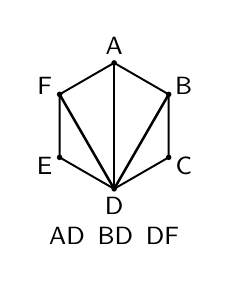
\begin{tikzpicture}[baseline=(current bounding box.center),every node/.style={font=\small}]
\coordinate (v0) at (0.0000,0.8000);
\coordinate (v1) at (0.6928,0.4000);
\coordinate (v2) at (0.6928,-0.4000);
\coordinate (v3) at (0.0000,-0.8000);
\coordinate (v4) at (-0.6928,-0.4000);
\coordinate (v5) at (-0.6928,0.4000);
\draw[line width=.7pt] (v0)--(v1)--(v2)--(v3)--(v4)--(v5)--cycle;
\draw[line width=.9pt](v0)--(v3);
\draw[line width=.9pt](v1)--(v3);
\draw[line width=.9pt](v3)--(v5);
\fill (v0) circle (1pt);\node at (0.0000,1.0200) {A};
\fill (v1) circle (1pt);\node at (0.8833,0.5100) {B};
\fill (v2) circle (1pt);\node at (0.8833,-0.5100) {C};
\fill (v3) circle (1pt);\node at (0.0000,-1.0200) {D};
\fill (v4) circle (1pt);\node at (-0.8833,-0.5100) {E};
\fill (v5) circle (1pt);\node at (-0.8833,0.5100) {F};
\node[align=center,font=\small] at (0,-1.400) {AD\, BD\, DF};
\end{tikzpicture} & 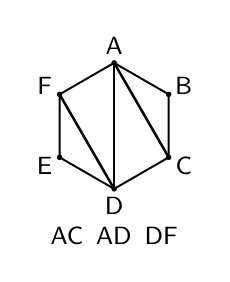
\begin{tikzpicture}[baseline=(current bounding box.center),every node/.style={font=\small}]
\coordinate (v0) at (0.0000,0.8000);
\coordinate (v1) at (0.6928,0.4000);
\coordinate (v2) at (0.6928,-0.4000);
\coordinate (v3) at (0.0000,-0.8000);
\coordinate (v4) at (-0.6928,-0.4000);
\coordinate (v5) at (-0.6928,0.4000);
\draw[line width=.7pt] (v0)--(v1)--(v2)--(v3)--(v4)--(v5)--cycle;
\draw[line width=.9pt](v0)--(v2);
\draw[line width=.9pt](v0)--(v3);
\draw[line width=.9pt](v3)--(v5);
\fill (v0) circle (1pt);\node at (0.0000,1.0200) {A};
\fill (v1) circle (1pt);\node at (0.8833,0.5100) {B};
\fill (v2) circle (1pt);\node at (0.8833,-0.5100) {C};
\fill (v3) circle (1pt);\node at (0.0000,-1.0200) {D};
\fill (v4) circle (1pt);\node at (-0.8833,-0.5100) {E};
\fill (v5) circle (1pt);\node at (-0.8833,0.5100) {F};
\node[align=center,font=\small] at (0,-1.400) {AC\, AD\, DF};
\end{tikzpicture}\\[7pt]
\end{tabular}\end{center}
\textbf{Third corner E: five fillings.} Triangle AEF leaves pentagon ABCDE.
\begin{center}\begin{tabular}{ccccc}
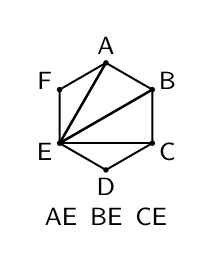
\begin{tikzpicture}[baseline=(current bounding box.center),every node/.style={font=\small}]
\coordinate (v0) at (0.0000,0.6800);
\coordinate (v1) at (0.5889,0.3400);
\coordinate (v2) at (0.5889,-0.3400);
\coordinate (v3) at (0.0000,-0.6800);
\coordinate (v4) at (-0.5889,-0.3400);
\coordinate (v5) at (-0.5889,0.3400);
\draw[line width=.7pt] (v0)--(v1)--(v2)--(v3)--(v4)--(v5)--cycle;
\draw[line width=.9pt](v0)--(v4);
\draw[line width=.9pt](v1)--(v4);
\draw[line width=.9pt](v2)--(v4);
\fill (v0) circle (1pt);\node at (0.0000,0.9000) {A};
\fill (v1) circle (1pt);\node at (0.7794,0.4500) {B};
\fill (v2) circle (1pt);\node at (0.7794,-0.4500) {C};
\fill (v3) circle (1pt);\node at (0.0000,-0.9000) {D};
\fill (v4) circle (1pt);\node at (-0.7794,-0.4500) {E};
\fill (v5) circle (1pt);\node at (-0.7794,0.4500) {F};
\node[align=center,font=\small] at (0,-1.280) {AE\, BE\, CE};
\end{tikzpicture} & 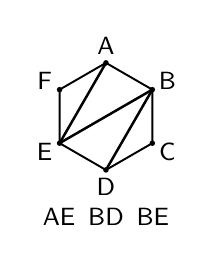
\begin{tikzpicture}[baseline=(current bounding box.center),every node/.style={font=\small}]
\coordinate (v0) at (0.0000,0.6800);
\coordinate (v1) at (0.5889,0.3400);
\coordinate (v2) at (0.5889,-0.3400);
\coordinate (v3) at (0.0000,-0.6800);
\coordinate (v4) at (-0.5889,-0.3400);
\coordinate (v5) at (-0.5889,0.3400);
\draw[line width=.7pt] (v0)--(v1)--(v2)--(v3)--(v4)--(v5)--cycle;
\draw[line width=.9pt](v0)--(v4);
\draw[line width=.9pt](v1)--(v3);
\draw[line width=.9pt](v1)--(v4);
\fill (v0) circle (1pt);\node at (0.0000,0.9000) {A};
\fill (v1) circle (1pt);\node at (0.7794,0.4500) {B};
\fill (v2) circle (1pt);\node at (0.7794,-0.4500) {C};
\fill (v3) circle (1pt);\node at (0.0000,-0.9000) {D};
\fill (v4) circle (1pt);\node at (-0.7794,-0.4500) {E};
\fill (v5) circle (1pt);\node at (-0.7794,0.4500) {F};
\node[align=center,font=\small] at (0,-1.280) {AE\, BD\, BE};
\end{tikzpicture} & 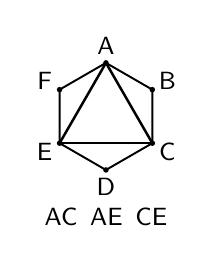
\begin{tikzpicture}[baseline=(current bounding box.center),every node/.style={font=\small}]
\coordinate (v0) at (0.0000,0.6800);
\coordinate (v1) at (0.5889,0.3400);
\coordinate (v2) at (0.5889,-0.3400);
\coordinate (v3) at (0.0000,-0.6800);
\coordinate (v4) at (-0.5889,-0.3400);
\coordinate (v5) at (-0.5889,0.3400);
\draw[line width=.7pt] (v0)--(v1)--(v2)--(v3)--(v4)--(v5)--cycle;
\draw[line width=.9pt](v0)--(v2);
\draw[line width=.9pt](v0)--(v4);
\draw[line width=.9pt](v2)--(v4);
\fill (v0) circle (1pt);\node at (0.0000,0.9000) {A};
\fill (v1) circle (1pt);\node at (0.7794,0.4500) {B};
\fill (v2) circle (1pt);\node at (0.7794,-0.4500) {C};
\fill (v3) circle (1pt);\node at (0.0000,-0.9000) {D};
\fill (v4) circle (1pt);\node at (-0.7794,-0.4500) {E};
\fill (v5) circle (1pt);\node at (-0.7794,0.4500) {F};
\node[align=center,font=\small] at (0,-1.280) {AC\, AE\, CE};
\end{tikzpicture} & 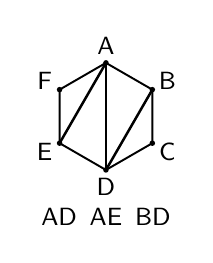
\begin{tikzpicture}[baseline=(current bounding box.center),every node/.style={font=\small}]
\coordinate (v0) at (0.0000,0.6800);
\coordinate (v1) at (0.5889,0.3400);
\coordinate (v2) at (0.5889,-0.3400);
\coordinate (v3) at (0.0000,-0.6800);
\coordinate (v4) at (-0.5889,-0.3400);
\coordinate (v5) at (-0.5889,0.3400);
\draw[line width=.7pt] (v0)--(v1)--(v2)--(v3)--(v4)--(v5)--cycle;
\draw[line width=.9pt](v0)--(v3);
\draw[line width=.9pt](v0)--(v4);
\draw[line width=.9pt](v1)--(v3);
\fill (v0) circle (1pt);\node at (0.0000,0.9000) {A};
\fill (v1) circle (1pt);\node at (0.7794,0.4500) {B};
\fill (v2) circle (1pt);\node at (0.7794,-0.4500) {C};
\fill (v3) circle (1pt);\node at (0.0000,-0.9000) {D};
\fill (v4) circle (1pt);\node at (-0.7794,-0.4500) {E};
\fill (v5) circle (1pt);\node at (-0.7794,0.4500) {F};
\node[align=center,font=\small] at (0,-1.280) {AD\, AE\, BD};
\end{tikzpicture} & 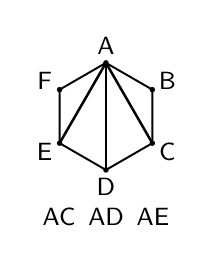
\begin{tikzpicture}[baseline=(current bounding box.center),every node/.style={font=\small}]
\coordinate (v0) at (0.0000,0.6800);
\coordinate (v1) at (0.5889,0.3400);
\coordinate (v2) at (0.5889,-0.3400);
\coordinate (v3) at (0.0000,-0.6800);
\coordinate (v4) at (-0.5889,-0.3400);
\coordinate (v5) at (-0.5889,0.3400);
\draw[line width=.7pt] (v0)--(v1)--(v2)--(v3)--(v4)--(v5)--cycle;
\draw[line width=.9pt](v0)--(v2);
\draw[line width=.9pt](v0)--(v3);
\draw[line width=.9pt](v0)--(v4);
\fill (v0) circle (1pt);\node at (0.0000,0.9000) {A};
\fill (v1) circle (1pt);\node at (0.7794,0.4500) {B};
\fill (v2) circle (1pt);\node at (0.7794,-0.4500) {C};
\fill (v3) circle (1pt);\node at (0.0000,-0.9000) {D};
\fill (v4) circle (1pt);\node at (-0.7794,-0.4500) {E};
\fill (v5) circle (1pt);\node at (-0.7794,0.4500) {F};
\node[align=center,font=\small] at (0,-1.280) {AC\, AD\, AE};
\end{tikzpicture}\\[7pt]
\end{tabular}\end{center}
\textbf{Why no omissions or repeats.} A filling has exactly one triangle touching AF. Its third corner assigns it to exactly one group. The remaining polygon pieces can be filled independently; their complete smaller lists give $5+2+2+5=14$. No filling belongs to two groups.
\hint{Let children collect freely first. When a collection is hard to audit, ask which triangle touches AF in each picture. The student pages offer 17 recording outlines; the number of blank spaces is not the answer.}

\newpage
\pagehead{Grades 4--5 solutions for Problems 1 to 4}
\prob{Problem 1}{The five pentagon fans on page 3 are the complete answer. The shared-corner proof or the root-edge classification proves no filling is missing.}
\prob{Problem 2}{The two printed hexagon starts have the same six neighbors keyed in middle P3 and pictured in K--1 P5. Each start has exactly three possible flips. The two-triangle quadrilateral argument on page 5 proves completeness.}
\hint{A different-looking triangulation need not be one move away. Check that exactly one old diagonal disappeared and exactly one new one appeared.}
\prob{Problem 3}{The complete map is the five-cycle on page 6. The five-flip loop $F_A,F_C,F_E,F_B,F_D,F_A$ is an odd return. Its reverse is also valid. The graph is not bipartite: alternating two colors around the cycle makes the final edge join two same-colored vertices.}
\textbf{Fidelity warning.} A parity invariant from lozenge tiling flips does not transfer here. The objects and moves are different; a polygon five-cycle is a direct counterexample to an even-return claim.
\prob{Problem 4}{The three starts, left to right, are $\{BD,BE,BF\}$, $\{AC,AE,CE\}$, and $\{AD,BD,DF\}$. The fourth filling is the A fan $\{AC,AD,AE\}$. Their minimum distances are 3, 1, and 2.}
\textbf{Left start.} Use the three-flip route on page 7: replace BF by AE, BE by AD, then BD by AC. It is shortest because all three target diagonals were missing.
\textbf{Middle start.} Replace CE by AD. Exactly one target diagonal was missing.
\begin{center}\begin{tabular}{cc}
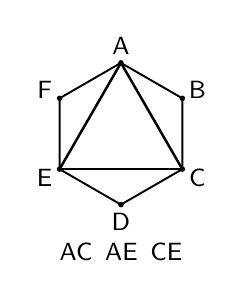
\begin{tikzpicture}[baseline=(current bounding box.center),every node/.style={font=\small}]
\coordinate (v0) at (0.0000,0.9000);
\coordinate (v1) at (0.7794,0.4500);
\coordinate (v2) at (0.7794,-0.4500);
\coordinate (v3) at (0.0000,-0.9000);
\coordinate (v4) at (-0.7794,-0.4500);
\coordinate (v5) at (-0.7794,0.4500);
\draw[line width=.7pt] (v0)--(v1)--(v2)--(v3)--(v4)--(v5)--cycle;
\draw[line width=.9pt](v0)--(v2);
\draw[line width=.9pt](v0)--(v4);
\draw[line width=.9pt](v2)--(v4);
\fill (v0) circle (1pt);\node at (0.0000,1.1200) {A};
\fill (v1) circle (1pt);\node at (0.9699,0.5600) {B};
\fill (v2) circle (1pt);\node at (0.9699,-0.5600) {C};
\fill (v3) circle (1pt);\node at (0.0000,-1.1200) {D};
\fill (v4) circle (1pt);\node at (-0.9699,-0.5600) {E};
\fill (v5) circle (1pt);\node at (-0.9699,0.5600) {F};
\node[align=center,font=\small] at (0,-1.500) {AC\, AE\, CE};
\end{tikzpicture} & 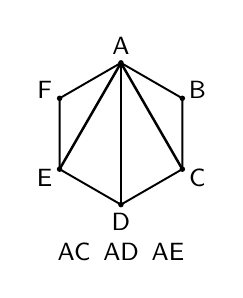
\begin{tikzpicture}[baseline=(current bounding box.center),every node/.style={font=\small}]
\coordinate (v0) at (0.0000,0.9000);
\coordinate (v1) at (0.7794,0.4500);
\coordinate (v2) at (0.7794,-0.4500);
\coordinate (v3) at (0.0000,-0.9000);
\coordinate (v4) at (-0.7794,-0.4500);
\coordinate (v5) at (-0.7794,0.4500);
\draw[line width=.7pt] (v0)--(v1)--(v2)--(v3)--(v4)--(v5)--cycle;
\draw[line width=.9pt](v0)--(v2);
\draw[line width=.9pt](v0)--(v3);
\draw[line width=.9pt](v0)--(v4);
\fill (v0) circle (1pt);\node at (0.0000,1.1200) {A};
\fill (v1) circle (1pt);\node at (0.9699,0.5600) {B};
\fill (v2) circle (1pt);\node at (0.9699,-0.5600) {C};
\fill (v3) circle (1pt);\node at (0.0000,-1.1200) {D};
\fill (v4) circle (1pt);\node at (-0.9699,-0.5600) {E};
\fill (v5) circle (1pt);\node at (-0.9699,0.5600) {F};
\node[align=center,font=\small] at (0,-1.500) {AC\, AD\, AE};
\end{tikzpicture}\\[7pt]
\end{tabular}\end{center}
\textbf{Right start.} Replace BD by AC, then DF by AE. Exactly two target diagonals were missing.
\begin{center}\begin{tabular}{ccc}
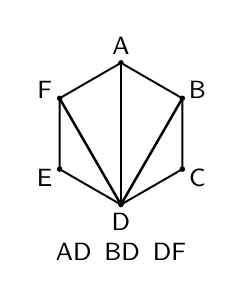
\begin{tikzpicture}[baseline=(current bounding box.center),every node/.style={font=\small}]
\coordinate (v0) at (0.0000,0.9000);
\coordinate (v1) at (0.7794,0.4500);
\coordinate (v2) at (0.7794,-0.4500);
\coordinate (v3) at (0.0000,-0.9000);
\coordinate (v4) at (-0.7794,-0.4500);
\coordinate (v5) at (-0.7794,0.4500);
\draw[line width=.7pt] (v0)--(v1)--(v2)--(v3)--(v4)--(v5)--cycle;
\draw[line width=.9pt](v0)--(v3);
\draw[line width=.9pt](v1)--(v3);
\draw[line width=.9pt](v3)--(v5);
\fill (v0) circle (1pt);\node at (0.0000,1.1200) {A};
\fill (v1) circle (1pt);\node at (0.9699,0.5600) {B};
\fill (v2) circle (1pt);\node at (0.9699,-0.5600) {C};
\fill (v3) circle (1pt);\node at (0.0000,-1.1200) {D};
\fill (v4) circle (1pt);\node at (-0.9699,-0.5600) {E};
\fill (v5) circle (1pt);\node at (-0.9699,0.5600) {F};
\node[align=center,font=\small] at (0,-1.500) {AD\, BD\, DF};
\end{tikzpicture} & 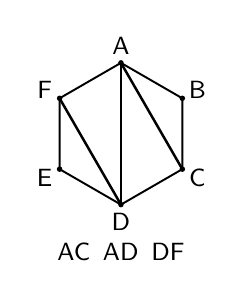
\begin{tikzpicture}[baseline=(current bounding box.center),every node/.style={font=\small}]
\coordinate (v0) at (0.0000,0.9000);
\coordinate (v1) at (0.7794,0.4500);
\coordinate (v2) at (0.7794,-0.4500);
\coordinate (v3) at (0.0000,-0.9000);
\coordinate (v4) at (-0.7794,-0.4500);
\coordinate (v5) at (-0.7794,0.4500);
\draw[line width=.7pt] (v0)--(v1)--(v2)--(v3)--(v4)--(v5)--cycle;
\draw[line width=.9pt](v0)--(v2);
\draw[line width=.9pt](v0)--(v3);
\draw[line width=.9pt](v3)--(v5);
\fill (v0) circle (1pt);\node at (0.0000,1.1200) {A};
\fill (v1) circle (1pt);\node at (0.9699,0.5600) {B};
\fill (v2) circle (1pt);\node at (0.9699,-0.5600) {C};
\fill (v3) circle (1pt);\node at (0.0000,-1.1200) {D};
\fill (v4) circle (1pt);\node at (-0.9699,-0.5600) {E};
\fill (v5) circle (1pt);\node at (-0.9699,0.5600) {F};
\node[align=center,font=\small] at (0,-1.500) {AC\, AD\, DF};
\end{tikzpicture} & 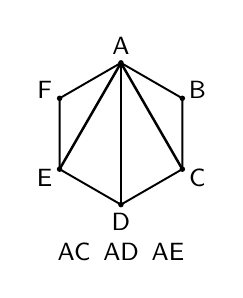
\begin{tikzpicture}[baseline=(current bounding box.center),every node/.style={font=\small}]
\coordinate (v0) at (0.0000,0.9000);
\coordinate (v1) at (0.7794,0.4500);
\coordinate (v2) at (0.7794,-0.4500);
\coordinate (v3) at (0.0000,-0.9000);
\coordinate (v4) at (-0.7794,-0.4500);
\coordinate (v5) at (-0.7794,0.4500);
\draw[line width=.7pt] (v0)--(v1)--(v2)--(v3)--(v4)--(v5)--cycle;
\draw[line width=.9pt](v0)--(v2);
\draw[line width=.9pt](v0)--(v3);
\draw[line width=.9pt](v0)--(v4);
\fill (v0) circle (1pt);\node at (0.0000,1.1200) {A};
\fill (v1) circle (1pt);\node at (0.9699,0.5600) {B};
\fill (v2) circle (1pt);\node at (0.9699,-0.5600) {C};
\fill (v3) circle (1pt);\node at (0.0000,-1.1200) {D};
\fill (v4) circle (1pt);\node at (-0.9699,-0.5600) {E};
\fill (v5) circle (1pt);\node at (-0.9699,0.5600) {F};
\node[align=center,font=\small] at (0,-1.500) {AC\, AD\, AE};
\end{tikzpicture}\\[7pt]
\end{tabular}\end{center}
\hint{Have a child mark which A-fan diagonals are already present, without erasing them. Ask how much that count can rise in one flip. A successful short route alone is not a proof that it is shortest.}

\newpage
\pagehead{Grades 4--5 Problem 5 and two octagon fans}
\prob{Problem 5}{The printed start is $S=\{AC,AD,DF,DG,DH\}$. A fan at A has five diagonals $\{AC,AD,AE,AF,AG\}$; a fan at E has $\{AE,BE,CE,EG,EH\}$. The minimum distances are 3 and 5, respectively.}
\begin{center}\begin{tabular}{ccc}
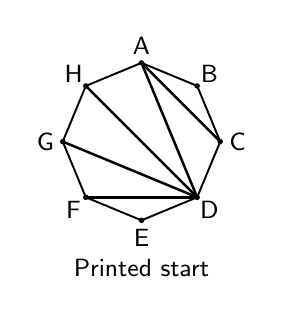
\begin{tikzpicture}[baseline=(current bounding box.center),every node/.style={font=\small}]
\coordinate (v0) at (0.0000,1.0000);
\coordinate (v1) at (0.7071,0.7071);
\coordinate (v2) at (1.0000,0.0000);
\coordinate (v3) at (0.7071,-0.7071);
\coordinate (v4) at (0.0000,-1.0000);
\coordinate (v5) at (-0.7071,-0.7071);
\coordinate (v6) at (-1.0000,-0.0000);
\coordinate (v7) at (-0.7071,0.7071);
\draw[line width=.7pt] (v0)--(v1)--(v2)--(v3)--(v4)--(v5)--(v6)--(v7)--cycle;
\draw[line width=.9pt](v0)--(v2);
\draw[line width=.9pt](v0)--(v3);
\draw[line width=.9pt](v3)--(v5);
\draw[line width=.9pt](v3)--(v6);
\draw[line width=.9pt](v3)--(v7);
\fill (v0) circle (1pt);\node at (0.0000,1.2200) {A};
\fill (v1) circle (1pt);\node at (0.8627,0.8627) {B};
\fill (v2) circle (1pt);\node at (1.2200,0.0000) {C};
\fill (v3) circle (1pt);\node at (0.8627,-0.8627) {D};
\fill (v4) circle (1pt);\node at (0.0000,-1.2200) {E};
\fill (v5) circle (1pt);\node at (-0.8627,-0.8627) {F};
\fill (v6) circle (1pt);\node at (-1.2200,-0.0000) {G};
\fill (v7) circle (1pt);\node at (-0.8627,0.8627) {H};
\node[align=center,font=\small] at (0,-1.600) {Printed start};
\end{tikzpicture} & 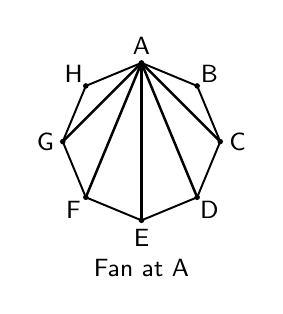
\begin{tikzpicture}[baseline=(current bounding box.center),every node/.style={font=\small}]
\coordinate (v0) at (0.0000,1.0000);
\coordinate (v1) at (0.7071,0.7071);
\coordinate (v2) at (1.0000,0.0000);
\coordinate (v3) at (0.7071,-0.7071);
\coordinate (v4) at (0.0000,-1.0000);
\coordinate (v5) at (-0.7071,-0.7071);
\coordinate (v6) at (-1.0000,-0.0000);
\coordinate (v7) at (-0.7071,0.7071);
\draw[line width=.7pt] (v0)--(v1)--(v2)--(v3)--(v4)--(v5)--(v6)--(v7)--cycle;
\draw[line width=.9pt](v0)--(v2);
\draw[line width=.9pt](v0)--(v3);
\draw[line width=.9pt](v0)--(v4);
\draw[line width=.9pt](v0)--(v5);
\draw[line width=.9pt](v0)--(v6);
\fill (v0) circle (1pt);\node at (0.0000,1.2200) {A};
\fill (v1) circle (1pt);\node at (0.8627,0.8627) {B};
\fill (v2) circle (1pt);\node at (1.2200,0.0000) {C};
\fill (v3) circle (1pt);\node at (0.8627,-0.8627) {D};
\fill (v4) circle (1pt);\node at (0.0000,-1.2200) {E};
\fill (v5) circle (1pt);\node at (-0.8627,-0.8627) {F};
\fill (v6) circle (1pt);\node at (-1.2200,-0.0000) {G};
\fill (v7) circle (1pt);\node at (-0.8627,0.8627) {H};
\node[align=center,font=\small] at (0,-1.600) {Fan at A};
\end{tikzpicture} & 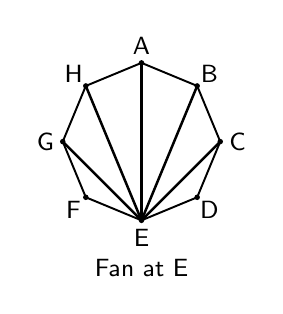
\begin{tikzpicture}[baseline=(current bounding box.center),every node/.style={font=\small}]
\coordinate (v0) at (0.0000,1.0000);
\coordinate (v1) at (0.7071,0.7071);
\coordinate (v2) at (1.0000,0.0000);
\coordinate (v3) at (0.7071,-0.7071);
\coordinate (v4) at (0.0000,-1.0000);
\coordinate (v5) at (-0.7071,-0.7071);
\coordinate (v6) at (-1.0000,-0.0000);
\coordinate (v7) at (-0.7071,0.7071);
\draw[line width=.7pt] (v0)--(v1)--(v2)--(v3)--(v4)--(v5)--(v6)--(v7)--cycle;
\draw[line width=.9pt](v0)--(v4);
\draw[line width=.9pt](v1)--(v4);
\draw[line width=.9pt](v2)--(v4);
\draw[line width=.9pt](v4)--(v6);
\draw[line width=.9pt](v4)--(v7);
\fill (v0) circle (1pt);\node at (0.0000,1.2200) {A};
\fill (v1) circle (1pt);\node at (0.8627,0.8627) {B};
\fill (v2) circle (1pt);\node at (1.2200,0.0000) {C};
\fill (v3) circle (1pt);\node at (0.8627,-0.8627) {D};
\fill (v4) circle (1pt);\node at (0.0000,-1.2200) {E};
\fill (v5) circle (1pt);\node at (-0.8627,-0.8627) {F};
\fill (v6) circle (1pt);\node at (-1.2200,-0.0000) {G};
\fill (v7) circle (1pt);\node at (-0.8627,0.8627) {H};
\node[align=center,font=\small] at (0,-1.600) {Fan at E};
\end{tikzpicture}\\[7pt]
\end{tabular}\end{center}
\textbf{Three-flip route to the A fan}
\begin{center}\begin{tabular}{rll}\toprule Step & Diagonals in the filling & Change just made\\\midrule
0 & AC, AD, DF, DG, DH & Start\\
1 & AC, AD, AG, DF, DG & DH $\to$ AG\\
2 & AC, AD, AF, AG, DF & DG $\to$ AF\\
3 & AC, AD, AE, AF, AG & DF $\to$ AE\\
\bottomrule\end{tabular}\end{center}

\textbf{Five-flip route to the E fan}
\begin{center}\begin{tabular}{rll}\toprule Step & Diagonals in the filling & Change just made\\\midrule
0 & AC, AD, DF, DG, DH & Start\\
1 & AC, AD, DG, DH, EG & DF $\to$ EG\\
2 & AC, AD, DH, EG, EH & DG $\to$ EH\\
3 & AC, AD, AE, EG, EH & DH $\to$ AE\\
4 & AC, AE, CE, EG, EH & AD $\to$ CE\\
5 & AE, BE, CE, EG, EH & AC $\to$ BE\\
\bottomrule\end{tabular}\end{center}

\textbf{Optimality certificates.} The start already has two of A's five diagonals and none of E's five. Each flip can add at most one target diagonal. Therefore at least $5-2=3$ and $5-0=5$ flips are required. Both tables achieve their lower bounds, always adding a target diagonal and never deleting one.
\hint{Ask the child to choose a target corner and point to every diagonal already meeting it. If a proposed flip removes one of those, ask whether a different choice can increase the count instead. The general reason that such a choice exists is on page 11.}
\textbf{Using the tables.} Step 0 is the given picture. Draw each later row on tracing paper and compare consecutive rows. The change column names the entire local move; all other diagonals stay fixed. The eight new pictures in the two routes fit the eight provided recording copies if the printed start is reused.

\newpage
\pagehead{Grades 4--5 Problem 6 and the fan rule}
\prob{Problem 6}{For a convex $n$-gon, let $d_A$ be the number of \emph{interior diagonals} in the starting filling incident to A. The minimum number of flips to the A fan is}
\[
\boxed{n-3-d_A}.
\]
Do not count the two boundary sides at A. For a triangle, $n-3=d_A=0$, so the formula includes the zero-move case.

\textbf{Lower bound.} Every filling has $n-3$ diagonals. An A fan has all of them incident to A. One flip adds at most one new A diagonal, so at least $n-3-d_A$ flips are necessary.

\textbf{Why that bound can always be attained.} Look at the union of all triangles touching A. If it is not the whole polygon, part of its boundary is an interior diagonal $uw$, with triangle $Auw$ on one side and a triangle $uwx$ on the other. Their union is a convex quadrilateral. Flip $uw$ to $Ax$. The old edge is not incident to A, and the new one is. The union of triangles at A grows, and the number of A diagonals rises by exactly one. Repeat until every diagonal meets A. There are exactly $n-3-d_A$ increases.
\begin{center}
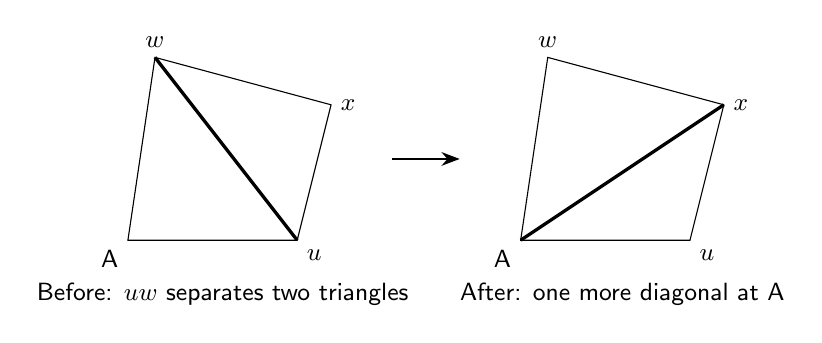
\begin{tikzpicture}[scale=.86,every node/.style={font=\small}]
\begin{scope}
\coordinate(a) at(0,0);\coordinate(u) at(2.5,0);\coordinate(x) at(3,2);\coordinate(w) at(.4,2.7);
\draw(a)--(u)--(x)--(w)--cycle;\draw[very thick](u)--(w);
\node[below left]at(a){A};\node[below right]at(u){$u$};\node[right]at(x){$x$};\node[above]at(w){$w$};
\node at(1.4,-.8){Before: $uw$ separates two triangles};
\end{scope}
\draw[-{Stealth},thick](3.9,1.2)--(4.9,1.2);
\begin{scope}[xshift=5.8cm]
\coordinate(a) at(0,0);\coordinate(u) at(2.5,0);\coordinate(x) at(3,2);\coordinate(w) at(.4,2.7);
\draw(a)--(u)--(x)--(w)--cycle;\draw[very thick](a)--(x);
\node[below left]at(a){A};\node[below right]at(u){$u$};\node[right]at(x){$x$};\node[above]at(w){$w$};
\node at(1.5,-.8){After: one more diagonal at A};
\end{scope}
\end{tikzpicture}
\end{center}
The picture is a local part of a larger polygon. Outside diagonals stay fixed. Strict convexity guarantees the other diagonal lies inside this quadrilateral.

\hint{First shade every triangle touching A on one concrete drawing. Ask where the shaded region could expand by changing one line. Once the child can do it twice, ask what would have to be true for the same move to be available again.}
\textbf{What constitutes an explanation.} ``I always add an A line'' is a useful strategy but incomplete unless the child explains why such a flip exists whenever some A lines are missing. The boundary-of-the-shaded-region argument supplies that missing step. The lower bound and construction have different jobs, and both are needed for an exact minimum.

\textbf{Why convexity matters.} In a nonconvex polygon, the union of two triangles need not be a convex quadrilateral; its other diagonal may leave the polygon. The guide's always-available flip argument is only for the strictly convex printed polygons.

\newpage
\pagehead{Grades 4--5 Problem 7 and connectivity}
\prob{Problem 7}{The printed endpoints are $S=\{AC,AD,DF,DG,DH\}$ and $T=\{AE,BD,BE,EG,EH\}$. Here is a five-flip route.}
\begin{center}\begin{tabular}{ccc}
\begin{tikzpicture}[baseline=(current bounding box.center),every node/.style={font=\small}]
\coordinate (v0) at (0.0000,0.8500);
\coordinate (v1) at (0.6010,0.6010);
\coordinate (v2) at (0.8500,0.0000);
\coordinate (v3) at (0.6010,-0.6010);
\coordinate (v4) at (0.0000,-0.8500);
\coordinate (v5) at (-0.6010,-0.6010);
\coordinate (v6) at (-0.8500,-0.0000);
\coordinate (v7) at (-0.6010,0.6010);
\draw[line width=.7pt] (v0)--(v1)--(v2)--(v3)--(v4)--(v5)--(v6)--(v7)--cycle;
\draw[line width=.9pt](v0)--(v2);
\draw[line width=.9pt](v0)--(v3);
\draw[line width=.9pt](v3)--(v5);
\draw[line width=.9pt](v3)--(v6);
\draw[line width=.9pt](v3)--(v7);
\fill (v0) circle (1pt);\node at (0.0000,1.0700) {A};
\fill (v1) circle (1pt);\node at (0.7566,0.7566) {B};
\fill (v2) circle (1pt);\node at (1.0700,0.0000) {C};
\fill (v3) circle (1pt);\node at (0.7566,-0.7566) {D};
\fill (v4) circle (1pt);\node at (0.0000,-1.0700) {E};
\fill (v5) circle (1pt);\node at (-0.7566,-0.7566) {F};
\fill (v6) circle (1pt);\node at (-1.0700,-0.0000) {G};
\fill (v7) circle (1pt);\node at (-0.7566,0.7566) {H};
\node[align=center,font=\small] at (0,-1.450) {Step 0};
\end{tikzpicture} & \begin{tikzpicture}[baseline=(current bounding box.center),every node/.style={font=\small}]
\coordinate (v0) at (0.0000,0.8500);
\coordinate (v1) at (0.6010,0.6010);
\coordinate (v2) at (0.8500,0.0000);
\coordinate (v3) at (0.6010,-0.6010);
\coordinate (v4) at (0.0000,-0.8500);
\coordinate (v5) at (-0.6010,-0.6010);
\coordinate (v6) at (-0.8500,-0.0000);
\coordinate (v7) at (-0.6010,0.6010);
\draw[line width=.7pt] (v0)--(v1)--(v2)--(v3)--(v4)--(v5)--(v6)--(v7)--cycle;
\draw[line width=.9pt](v0)--(v3);
\draw[line width=.9pt](v1)--(v3);
\draw[line width=.9pt](v3)--(v5);
\draw[line width=.9pt](v3)--(v6);
\draw[line width=.9pt](v3)--(v7);
\fill (v0) circle (1pt);\node at (0.0000,1.0700) {A};
\fill (v1) circle (1pt);\node at (0.7566,0.7566) {B};
\fill (v2) circle (1pt);\node at (1.0700,0.0000) {C};
\fill (v3) circle (1pt);\node at (0.7566,-0.7566) {D};
\fill (v4) circle (1pt);\node at (0.0000,-1.0700) {E};
\fill (v5) circle (1pt);\node at (-0.7566,-0.7566) {F};
\fill (v6) circle (1pt);\node at (-1.0700,-0.0000) {G};
\fill (v7) circle (1pt);\node at (-0.7566,0.7566) {H};
\node[align=center,font=\small] at (0,-1.450) {Step 1};
\end{tikzpicture} & \begin{tikzpicture}[baseline=(current bounding box.center),every node/.style={font=\small}]
\coordinate (v0) at (0.0000,0.8500);
\coordinate (v1) at (0.6010,0.6010);
\coordinate (v2) at (0.8500,0.0000);
\coordinate (v3) at (0.6010,-0.6010);
\coordinate (v4) at (0.0000,-0.8500);
\coordinate (v5) at (-0.6010,-0.6010);
\coordinate (v6) at (-0.8500,-0.0000);
\coordinate (v7) at (-0.6010,0.6010);
\draw[line width=.7pt] (v0)--(v1)--(v2)--(v3)--(v4)--(v5)--(v6)--(v7)--cycle;
\draw[line width=.9pt](v0)--(v3);
\draw[line width=.9pt](v1)--(v3);
\draw[line width=.9pt](v3)--(v6);
\draw[line width=.9pt](v3)--(v7);
\draw[line width=.9pt](v4)--(v6);
\fill (v0) circle (1pt);\node at (0.0000,1.0700) {A};
\fill (v1) circle (1pt);\node at (0.7566,0.7566) {B};
\fill (v2) circle (1pt);\node at (1.0700,0.0000) {C};
\fill (v3) circle (1pt);\node at (0.7566,-0.7566) {D};
\fill (v4) circle (1pt);\node at (0.0000,-1.0700) {E};
\fill (v5) circle (1pt);\node at (-0.7566,-0.7566) {F};
\fill (v6) circle (1pt);\node at (-1.0700,-0.0000) {G};
\fill (v7) circle (1pt);\node at (-0.7566,0.7566) {H};
\node[align=center,font=\small] at (0,-1.450) {Step 2};
\end{tikzpicture}\\[7pt]
\begin{tikzpicture}[baseline=(current bounding box.center),every node/.style={font=\small}]
\coordinate (v0) at (0.0000,0.8500);
\coordinate (v1) at (0.6010,0.6010);
\coordinate (v2) at (0.8500,0.0000);
\coordinate (v3) at (0.6010,-0.6010);
\coordinate (v4) at (0.0000,-0.8500);
\coordinate (v5) at (-0.6010,-0.6010);
\coordinate (v6) at (-0.8500,-0.0000);
\coordinate (v7) at (-0.6010,0.6010);
\draw[line width=.7pt] (v0)--(v1)--(v2)--(v3)--(v4)--(v5)--(v6)--(v7)--cycle;
\draw[line width=.9pt](v0)--(v3);
\draw[line width=.9pt](v1)--(v3);
\draw[line width=.9pt](v3)--(v7);
\draw[line width=.9pt](v4)--(v6);
\draw[line width=.9pt](v4)--(v7);
\fill (v0) circle (1pt);\node at (0.0000,1.0700) {A};
\fill (v1) circle (1pt);\node at (0.7566,0.7566) {B};
\fill (v2) circle (1pt);\node at (1.0700,0.0000) {C};
\fill (v3) circle (1pt);\node at (0.7566,-0.7566) {D};
\fill (v4) circle (1pt);\node at (0.0000,-1.0700) {E};
\fill (v5) circle (1pt);\node at (-0.7566,-0.7566) {F};
\fill (v6) circle (1pt);\node at (-1.0700,-0.0000) {G};
\fill (v7) circle (1pt);\node at (-0.7566,0.7566) {H};
\node[align=center,font=\small] at (0,-1.450) {Step 3};
\end{tikzpicture} & \begin{tikzpicture}[baseline=(current bounding box.center),every node/.style={font=\small}]
\coordinate (v0) at (0.0000,0.8500);
\coordinate (v1) at (0.6010,0.6010);
\coordinate (v2) at (0.8500,0.0000);
\coordinate (v3) at (0.6010,-0.6010);
\coordinate (v4) at (0.0000,-0.8500);
\coordinate (v5) at (-0.6010,-0.6010);
\coordinate (v6) at (-0.8500,-0.0000);
\coordinate (v7) at (-0.6010,0.6010);
\draw[line width=.7pt] (v0)--(v1)--(v2)--(v3)--(v4)--(v5)--(v6)--(v7)--cycle;
\draw[line width=.9pt](v0)--(v3);
\draw[line width=.9pt](v0)--(v4);
\draw[line width=.9pt](v1)--(v3);
\draw[line width=.9pt](v4)--(v6);
\draw[line width=.9pt](v4)--(v7);
\fill (v0) circle (1pt);\node at (0.0000,1.0700) {A};
\fill (v1) circle (1pt);\node at (0.7566,0.7566) {B};
\fill (v2) circle (1pt);\node at (1.0700,0.0000) {C};
\fill (v3) circle (1pt);\node at (0.7566,-0.7566) {D};
\fill (v4) circle (1pt);\node at (0.0000,-1.0700) {E};
\fill (v5) circle (1pt);\node at (-0.7566,-0.7566) {F};
\fill (v6) circle (1pt);\node at (-1.0700,-0.0000) {G};
\fill (v7) circle (1pt);\node at (-0.7566,0.7566) {H};
\node[align=center,font=\small] at (0,-1.450) {Step 4};
\end{tikzpicture} & \begin{tikzpicture}[baseline=(current bounding box.center),every node/.style={font=\small}]
\coordinate (v0) at (0.0000,0.8500);
\coordinate (v1) at (0.6010,0.6010);
\coordinate (v2) at (0.8500,0.0000);
\coordinate (v3) at (0.6010,-0.6010);
\coordinate (v4) at (0.0000,-0.8500);
\coordinate (v5) at (-0.6010,-0.6010);
\coordinate (v6) at (-0.8500,-0.0000);
\coordinate (v7) at (-0.6010,0.6010);
\draw[line width=.7pt] (v0)--(v1)--(v2)--(v3)--(v4)--(v5)--(v6)--(v7)--cycle;
\draw[line width=.9pt](v0)--(v4);
\draw[line width=.9pt](v1)--(v3);
\draw[line width=.9pt](v1)--(v4);
\draw[line width=.9pt](v4)--(v6);
\draw[line width=.9pt](v4)--(v7);
\fill (v0) circle (1pt);\node at (0.0000,1.0700) {A};
\fill (v1) circle (1pt);\node at (0.7566,0.7566) {B};
\fill (v2) circle (1pt);\node at (1.0700,0.0000) {C};
\fill (v3) circle (1pt);\node at (0.7566,-0.7566) {D};
\fill (v4) circle (1pt);\node at (0.0000,-1.0700) {E};
\fill (v5) circle (1pt);\node at (-0.7566,-0.7566) {F};
\fill (v6) circle (1pt);\node at (-1.0700,-0.0000) {G};
\fill (v7) circle (1pt);\node at (-0.7566,0.7566) {H};
\node[align=center,font=\small] at (0,-1.450) {Step 5};
\end{tikzpicture}\\[7pt]
\end{tabular}\end{center}
\begin{center}\begin{tabular}{rll}\toprule Step & Diagonals in the filling & Change just made\\\midrule
0 & AC, AD, DF, DG, DH & Start\\
1 & AD, BD, DF, DG, DH & AC $\to$ BD\\
2 & AD, BD, DG, DH, EG & DF $\to$ EG\\
3 & AD, BD, DH, EG, EH & DG $\to$ EH\\
4 & AD, AE, BD, EG, EH & DH $\to$ AE\\
5 & AE, BD, BE, EG, EH & AD $\to$ BE\\
\bottomrule\end{tabular}\end{center}

This route is also shortest, although the problem does not ask for that: the endpoints share no diagonal, so all five target diagonals must be introduced and one move adds at most one.

\textbf{Why any two fillings can be joined.} Choose one fixed corner, say A. Page 11's growing-fan procedure turns the first filling into the A fan and the second filling into the same A fan. Reverse the second route and place it after the first. Every reversed flip is legal, since exchanging the two diagonals of a convex quadrilateral is reversible. This gives a route between the original fillings. It need not be shortest.
\hint{If children can reach a fan but cannot connect arbitrary endpoints, ask whether a route can be followed backward. Be explicit that the same target corner must be used for both routes.}
\textbf{An upper bound, not an exact distance.} Passing through one fan uses $(n-3-d_A(S))+(n-3-d_A(T))$ flips. For these endpoints A gives $3+4=7$, while the route above uses 5. This example shows why a connectivity construction should not automatically be called a shortest route.

\newpage
\pagehead{Extensions sources and verification}
\textbf{Extensions with clear endpoints}
\begin{itemize}
\item Find the two fillings of a quadrilateral and their flip map. It has two vertices and one edge; every return walk is even. Compare this with the pentagon five-cycle. Odd return behavior depends on the configuration graph.
\item Choose boundary edge AF of the hexagon and count by its incident triangle. Then repeat the idea on a heptagon: the five possible third corners give $14+5+4+5+14=42$ fillings. Children may explain the products using independent polygon pieces; do not require the formula first.
\item Generalize that decomposition. If $T_n$ counts $n$-gon fillings and $T_2=1$ represents an empty side of a root triangle, then $T_n=\sum_{k=1}^{n-2}T_{k+1}T_{n-k}$. With $C_m=T_{m+2}$, this is $C_0=1$ and $C_{m+1}=\sum_{i=0}^{m}C_iC_{m-i}$. The empty-piece convention is a counting tool, not a claim that a two-sided polygon exists.
\item For a nonfan target, the missing-diagonal bound can be strict. From $\{BF,CE,CF\}$ to $\{AD,AE,BD\}$, all three target lines are missing, but the first flip can add only DF, BE, or AC, none of them a target line. At least four flips are needed. Four suffice via $\{BF,CF,DF\}$, then $\{BD,BF,DF\}$, then $\{AD,BD,DF\}$, then the target.
\end{itemize}
\textbf{Sources and exact scope}
\begin{itemize}
\item Richard P. Stanley, \emph{Catalan Numbers}, Tsuda slides (2017), PDF pp. 16--18 and 26--28, for polygon counts and the root-edge decomposition: \url{https://math.mit.edu/~rstan/transparencies/tsuda.pdf}.
\item Vincent Pilaud, \emph{Multitriangulations, pseudotriangulations and some problems of realization of polytopes}, Chapter 1, \S1.1, Lemma 1.2 and Proposition 1.4; printed pp. 51--53, PDF pp. 68--71, for triangle counts and the fan connectivity argument: \url{https://www.ub.edu/comb/vincentpilaud/documents/reports/theseVincentPilaud.pdf}.
\item Givental, Nemirovskaya, and Zakharevich, \emph{Math Circle by the Bay} (AMS, 2018), Preface pp. vii--ix. Its concrete manipulatives, student interaction, fallback hints, and repeated attention to explanations informed the adult support here. The exact menu and launch are local suggestions.
\end{itemize}
These are mathematical and pedagogical background sources, not classroom trials of these worksheets. Specific configurations, full answer catalogs, shortest routes, hints, and diagrams here were made for the final packet. Associahedra, parenthesizations, and generalized triangulations are not student prerequisites. The result assumes fixed labeled corners, straight diagonals, no added vertices, and strict convexity. Counts would change under different equivalences or allowed moves.

\textbf{Independent checks.} Root-edge recursion generated all triangulations for 3 through 8 corners, with counts 1, 2, 5, 14, 42, 132. Breadth-first search checked every printed route example and every fan distance through eight corners. Each listed route was checked for legal successive flips; the alternative middle route has no repeats. The checks were written independently of worksheet builders and draft count files. General proofs, rather than finite testing, support claims for all polygon sizes.

\textbf{After use.} Record which problems children actually attempted, whether labels remained fixed, whether the flip action was clear, which hints helped, and any explanation worth preserving. Do not mark the material piloted until that classroom evidence exists.

\end{document}
